\documentclass[conference,compsoc]{IEEEtran}
\usepackage{graphicx}
\usepackage{caption}

% *** SUBFIGURE PACKAGES ***
\usepackage{subfig}

\usepackage{blindtext}
\usepackage{adjustbox}
\usepackage{multirow}
\usepackage{color}
\usepackage{booktabs}
\usepackage{tabularx}
\usepackage{colortbl}
\usepackage{bbding}
\usepackage{tikz}
\usepackage{listings}
\usepackage{etoolbox}
\usepackage{subfig}

\usepackage{url}
\usepackage{setspace}
%\usepackage{enumitem}
\usepackage[british,english]{babel}


%\usepackage[caption=false,font=footnotesize]{subfig}


\newcommand{\circled}[2][]{\tikz[baseline=(char.base)]
    {\node[shape = circle, draw, inner sep = 1pt]
    (char) {\phantom{\ifblank{#1}{#2}{#1}}};%
    \node at (char.center) {\makebox[0pt][c]{#2}};}}
\robustify{\circled}


\newcommand\FIXME[1]{\textcolor{red}{FIX:}\textcolor{red}{#1}}

\makeatletter
\def\@IEEEsectpunct{.\ \,}
\def\paragraph{\@startsection{paragraph}{4}{\z@}{1.5ex plus 1.5ex minus 0.5ex}%
{0ex}{\normalfont\normalsize\sffamily\bfseries}}


\patchcmd{\@maketitle}
  {\addvspace{0.2\baselineskip}\egroup}
  {\addvspace{-1\baselineskip}\egroup}


\makeatother

\newcommand{\cparagraph}[1]{\vspace{1mm}\noindent \textbf{#1}}



\newcommand{\topone} {{top-1}\xspace}
\newcommand{\topfive} {{top-5}\xspace}
\newcommand{\DNN} {\texttt{DNN}\xspace}
\newcommand{\DNNs} {\texttt{DNNs}\xspace}
\newcommand{\CNN} {\texttt{CNN}\xspace}
\newcommand{\RNN} {\texttt{RNN}\xspace}
\newcommand{\RNNs} {\texttt{RNNs}\xspace}
\newcommand{\CNNs} {\texttt{CNNs}\xspace}
\newcommand{\NN} {\texttt{KNN}\xspace}
\newcommand{\nNN} {\texttt{NN}\xspace}
\newcommand{\SVM} {\texttt{SVM}\xspace}
\newcommand{\DT} {\texttt{DT}\xspace}

\usepackage{multirow}

\begin{document}
%
% paper title
% Titles are generally capitalized except for words such as a, an, and, as,
% at, but, by, for, in, nor, of, on, or, the, to and up, which are usually
% not capitalized unless they are the first or last word of the title.
% Linebreaks \\ can be used within to get better formatting as desired.
% Do not put math or special symbols in the title.
\title{Network Delay-Aware Optimization for Web Browsing \\on Heterogeneous Mobile Platforms\vspace{-4 mm}}

 
\author{\IEEEauthorblockN{Jie Ren\IEEEauthorrefmark{2}, Xiaoming Wang\IEEEauthorrefmark{2}, Feng Tian\IEEEauthorrefmark{2},  Hai Wang\IEEEauthorrefmark{3},
 Jie Zheng\IEEEauthorrefmark{3}, Zheng Wang\IEEEauthorrefmark{1}} \IEEEauthorblockA{
\IEEEauthorrefmark{2} Shaanxi Normal University, China, \IEEEauthorrefmark{3}Northwest University, China, \IEEEauthorrefmark{1}Lancaster University, UK \\
\IEEEauthorrefmark{2}\{renjie, wangxm, tianfeng\}@snnu.edu.cn, \IEEEauthorrefmark{3}\{hwang, jzheng\}@nwu.edu.cn,
\IEEEauthorrefmark{1}z.wang@lancaster.ac.uk \vspace{-4 mm} } }

% make the title area
\maketitle

% As a general rule, do not put math, special symbols or citations
% in the abstract
\begin{abstract}
In this paper, we propose a machine
learning based approach to predict which of the heterogeneous processors to use to render the web content and the operating frequencies of heterogeneous processors.
We do so by first learning, \emph{offline}, a set of predictive models for a range of networking
environments. We then choose a learnt model at runtime to predict the optimal processor configuration. The prediction is based on the web content, the network status and the optimization goal.
We obtain, on average, over 21\% and 39\%
of improvement respectively for load time and energy consumption, when compared to two competitive
optimisers that are specifically tuned for mobile web browsing.
\end{abstract}





% For peer review papers, you can put extra information on the cover
% page as needed:
% \ifCLASSOPTIONpeerreview
% \begin{center} \bfseries EDICS Category: 3-BBND \end{center}
% \fi
%
% For peerreview papers, this IEEEtran command inserts a page break and
% creates the second title. It will be ignored for other modes.
\IEEEpeerreviewmaketitle

\section{Introduction}
In recent years, deep learning has emerged as a powerful tool for solving problems that were considered to be difficult in the past. It has
demonstrated impressive results on tasks like object recognition~\cite{donahue14,he2016deep}, facial
recognition~\cite{parkhi2015deep,sun2014deep}, speech processing~\cite{pmlrv48amodei16}, and machine translation~\cite{bahdanau2014neural}.
While many of these tasks are also important on mobiles and the Internet of Things (IoT), existing solutions are often
computation-intensive and require a large amount of resources for the model to operate. Performing deep inference\footnote{Inference in
this paper refers to apply a pre-trained model on an input to obtain the corresponding output. This is different from statistical
inference.} on embedded devices can lead to long runtimes and the consumption of abundant amounts of resources, including CPU, memory, and
power, even for simple tasks~\cite{CanzianiPC16}. Without a solution,
 the hoped-for advances on embedded sensing will not arrive.


Numerous approaches have been proposed to accelerate deep inference on embedded devices. These include designing specialize hardware to
reduce the computation or memory latency~\cite{}, compressing a pre-trained model to reduce its storage and memory footprint as well as
computational requirements~\cite{}, and offloading some, or all, computation to a cloud
server~\cite{Kang2017neurosurgeon,teerapittayanon2017distributed}. Compared to specialized hardware, software-based model compression
techniques have the advantage of being readily deployable on commercial-off-the-self hardware and compared to computation offloading, model
compression enables on-device inference which in turn allows faster response time and has less privacy concerns. These advantages make
model compressions attractive on existing hardware platform where computation offloading is not feasible.


However, model compression is not a free lunch as it comes at the cost of loss in prediction accuracy~\cite{}. This means that one must
carefully choose the model compression technique and its parameters to effectively trade precision for computation and resource
requirements. Furthermore, as we will show in this paper, the reduction in the model size does not necessarily translate into faster
inference time. Because a model compression technique is not always beneficial, it is important to understand when and how to apply a
 technique.

In this paper, we aim to understand model compression techniques for embedded inference. Having this knowledge allows not only better
deployment of computation-intensive models on mobile and IoT devices, but also designing more efficient architectures for models and
hardware acceleration.

In this work, we conducted extensive experiments to evaluate two mainstream model compression techniques, pruning~\cite{Li2016Pruning} and data
quantization~\cite{Gong2014Compressing}. We apply model compression techniques to the image classification domain, an area where deep learning has made
impressive breakthroughs and a rich set of pre-trained models are available. We evaluate our approach on the NVIDIA Jetson TX2 embedded
deep learning platform and consider a wide range of influential DNN models. Our experiments are performed using the 50K images from the
ImageNet ILSVRC 2012 validation dataset.

We show that while there may be significant gain for choosing the right compression technique and parameters, mistakes can seriously hurt
the performance. We show how different model compression techniques and parameters affect the inference time, model storage requirement and
the prediction accuracy. As a result, our work provides insights on when and how to apply deep learning model compression techniques on
embedded devices.

The main contributions of this paper are two folds:

\begin{itemize}
\item We present an extensive study to characterize and understand how two popular model compression techniques perform on a
    representative embedded deep learning platform;
\item Our work offers insights on when and how to apply compression techniques for embedded deep inference.
\end{itemize}

\section{Motivation}


%The JavaScript engine's performance that involves the compiler,
%garbage collector, etc., and the final display work on GPU are separate issues beyond the scope of this work.

\begin{table}[!t]
\caption{The best-performing available governor}
\vspace{-3mm}
\scriptsize
\begin{center}
        \begin{tabular}{llll}
        \toprule
        &\textbf{Load time}&\textbf{Energy}&\textbf{EDP}\\
        \midrule
            Regular 3G                     &\Performance&\Powersave&\Powersave\\
            \rowcolor{Gray}Regular 4G                     &\Performance&\Conservative&\Interactive\\
            WiFi            &\Interactive&\Ondemand&\Interactive\\
        \bottomrule
        \end{tabular}
\end{center}
\label{tab:best-governor}
\vspace{-5mm}
\end{table}


\begin{figure}[!t]
	\centering
	\subfloat[][Load time]{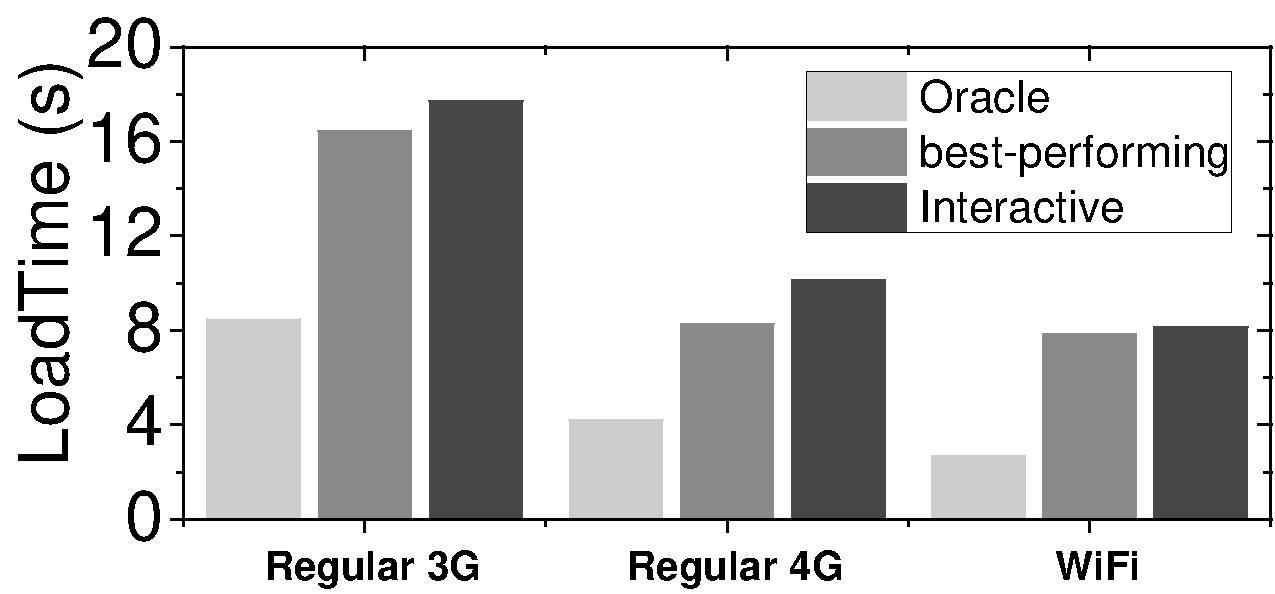
\includegraphics[width=0.22\textwidth]{figure/laod4pagesloadtime.pdf}}
    \hfill
    \subfloat[][Energy consumption]{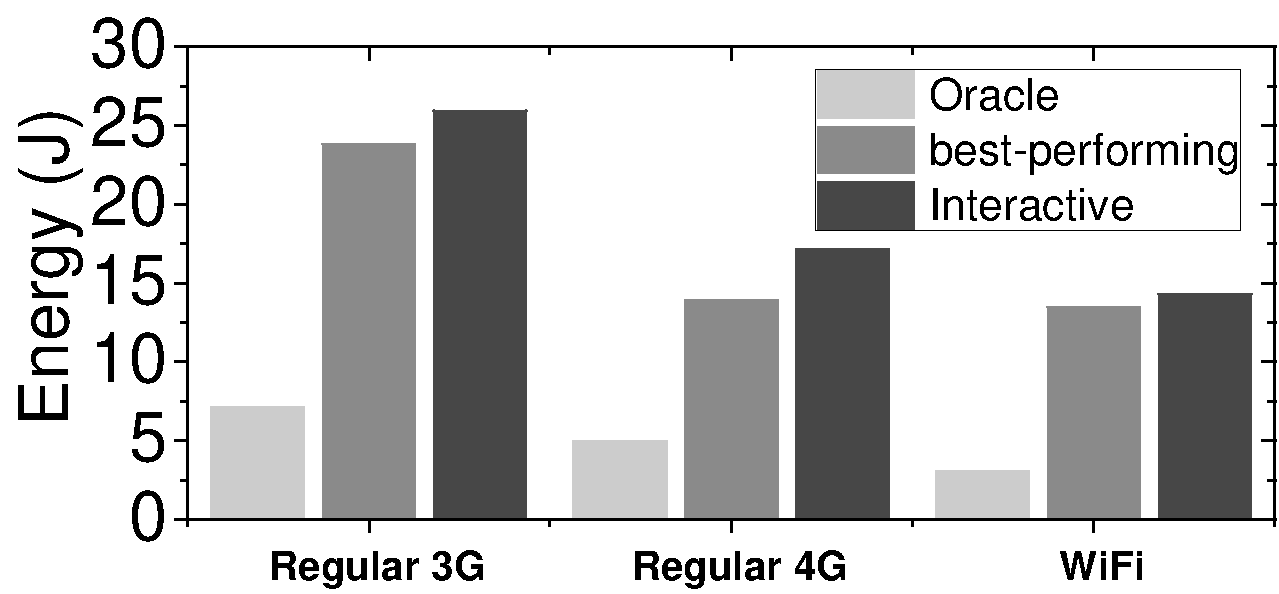
\includegraphics[width=0.22\textwidth]{figure/load4pagesEnergy.pdf}}
    \vspace{-2mm}
    \caption{The achieved total load time (a), energy consumption (b)  when a user was browsing four news pages from \BBCW.
    We show the results for \Oracle, the \bfp existing CPU frequency governor, and \Interactive in three typical networking environments. There is significant room for improvement. }
    \vspace{-5mm}
    \label{fig:motivation}
\end{figure}



Consider a scenario for browsing four \texttt{BBC} news pages, starting from the home page of \BBCW. Our evaluation platform has  a
Cortex-A15 (big) and a Cortex-A7 (little) processors.

\vspace{-1mm}
\cparagraph{Networking Environments.} We consider three typical networking
environments: Regular 3G, Regular 4G and WiFi (see Section~\ref{sec:networks} for more details). To ensure reproducible results, web requests and responses are deterministically replayed by the client and a web server respectively. The
web server simulates the download speed and latency of a given network setting, and we record and deterministically replay the
user interaction trace for each testing scenario.


\vspace{-1mm}
\cparagraph{Scheduling Strategies.} We schedule the Chromium rendering engine (i.e., \texttt{CrRendererMain}) to run on either the big or the little
core under different clock frequencies to find the best processor configuration per test case. We refer this best-found configuration as
the \Oracle because it is the best performance we can get via CPU frequency scaling and task mapping. We use the \Interactive CPU
frequency governor as the baseline, which is the default frequency governor on many mobile devices \cite{Seo2015Big}. We also compare with the best-performing governor found from mainstream CPU governors,
including
the \Interactive and other four strategies: \Performance, \Conservative, \Ondemand and \Powersave.


 %We evaluate the performance of each strategy in three typical networking environments, Regular 3G, Regular 4G,
%and WiFi, where a typical smartphone user would  experience. Table~\ref{tab:network} shows the configuration of each networking environment setting.
%Later in this paper, we evaluate our approach on a wider range of networking environments (see Section~\ref{}).

\cparagraph{Motivation Results.} Table~\ref{tab:best-governor} lists the best-performing governor chosen from the five existing CPU
frequency governors, and Figure~\ref{fig:motivation} summarizes the performance of each strategy for each optimization metric. While
\Interactive  gives the best \EDP compared to other existing governors in a Regular 4G and a WiFi environments, it fails to deliver the
best-available performance for load time and energy consumption. Furthermore, there is significant room for improvement for the best-performing
existing governor when compared to the \Oracle.  On average, the \Oracle outperforms the best-performing governor by 154.6\%,
70.6\% respectively for load time and energy consumption across networking environments.
More importantly, the oracle processor configuration varies across web pages, networking
environments and evaluation metrics -- no single configuration consistently delivers the best-available performance.

\cparagraph{Lessons Learned.} This example shows that the current mainstream CPU frequency governors are ill-suited for mobile web browsing
and the best processor configuration depends on the network and the optimization goal. There is a need for a better scheduler that can
adapt to the webpage workload, the networking environment and the optimization goal. In the remainder of this article, we describe such an
approach based on machine learning.

\section{Overview of our approach}

\begin{figure}
\begin{center}
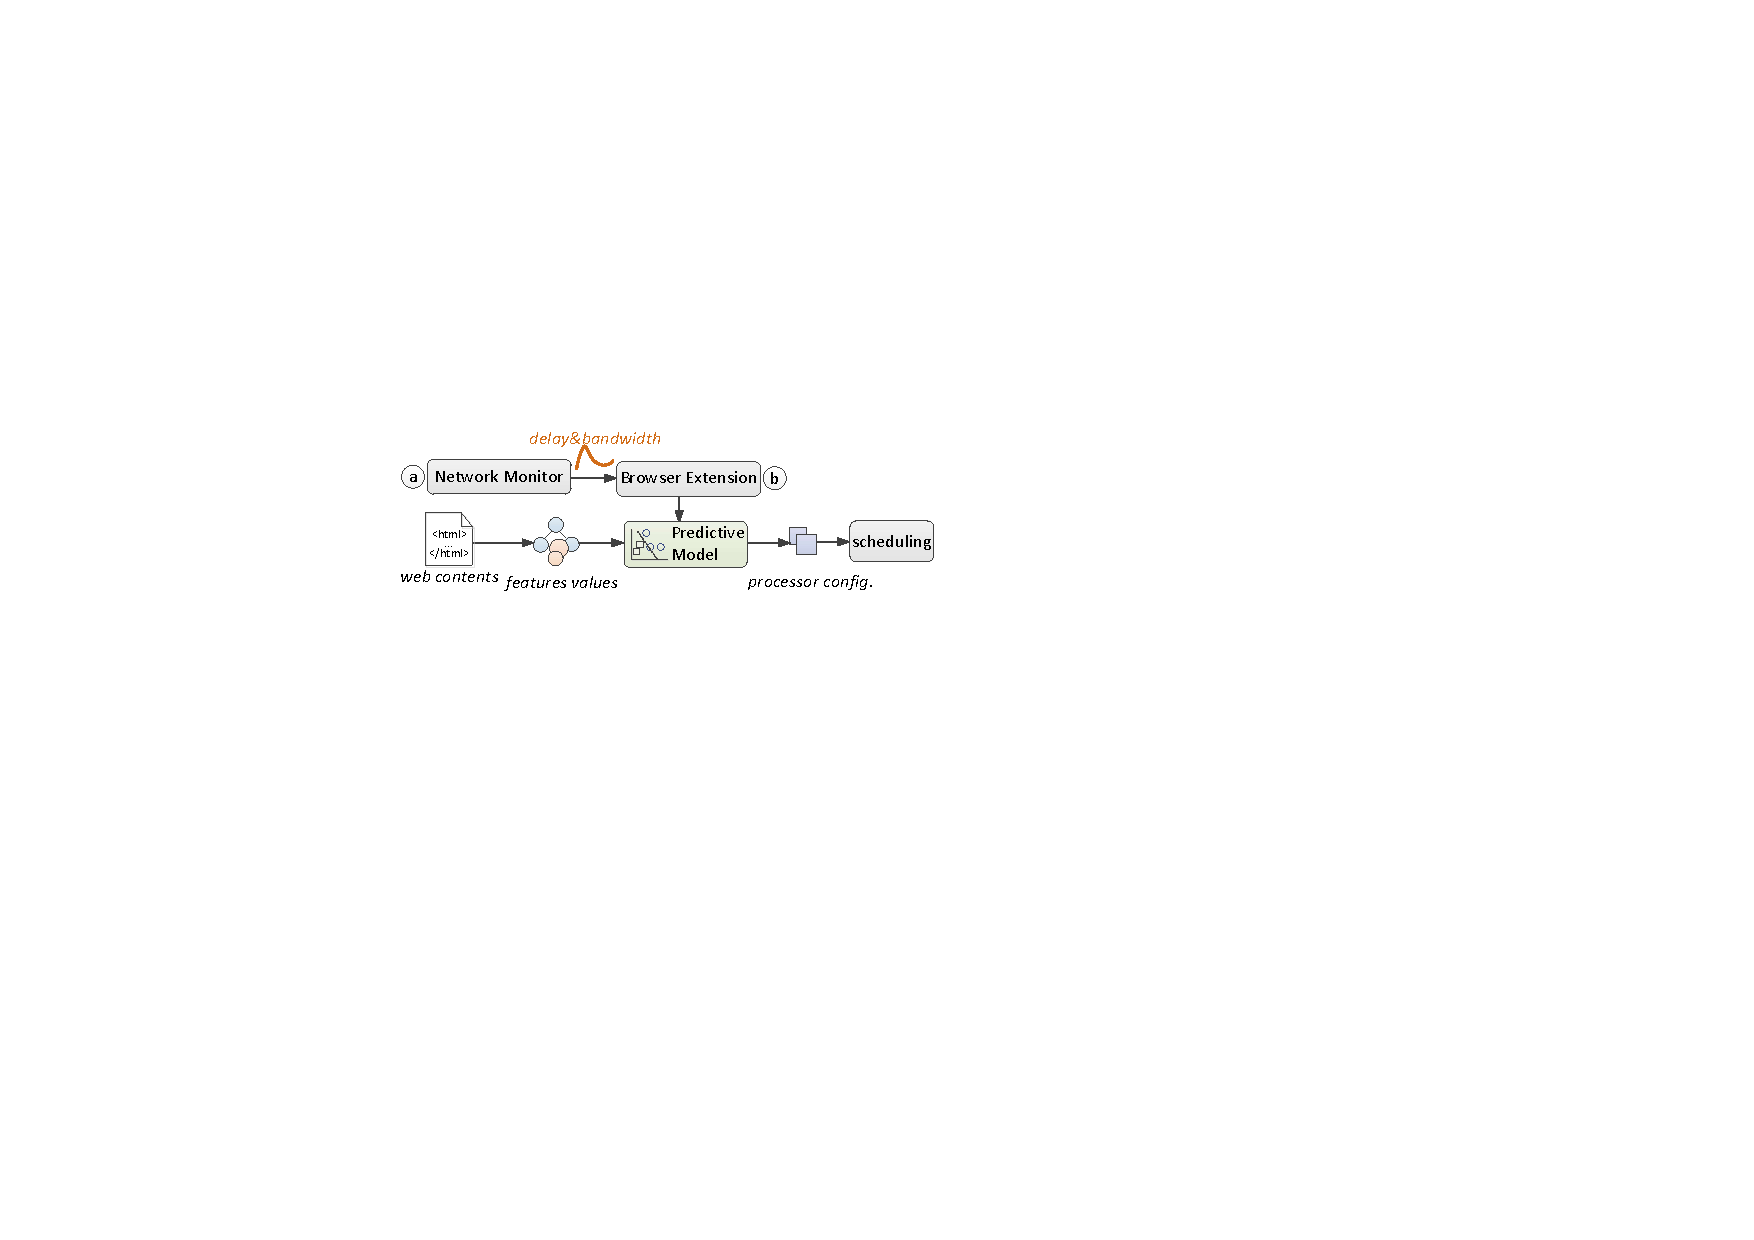
\includegraphics[width=0.5\textwidth]{figure/predictor.pdf}
\end{center}
\caption{Overview of our approach. The network monitor evaluates the network bandwidth and delay to choose a model to predict the
optimum processor configuration. }
\vspace{-4mm}
\label{fig:predictor}
\end{figure}


%Our goal is to develop a better CPU frequency governor to determine which of the multi-core processors to use to run the bowser rendering
%process and at what frequency the heterogeneous processor cores should operate. We target the ARM big.LITTLE heterogeneous multi-core
%architecture as it is now a commonplace on modern mobile devices. Rather than developing a hand-crafted approach that requires expert insight
%into the relative costs and idiosyncrasies of a particular platform and networking environment, we develop an automatic technique that is
%independent of the computing environment.


%We achieve this by employing machine learning to automatically build
%\emph{off-line} models of the platform's behavior, based on prior training data. The learnt models then predicts the best CPU frequency
%decision for any \emph{unseen} webpage in a given networking environment.

As illustrated in Figure~\ref{fig:predictor}, our approach consists of two components: (i) a network monitor running as an operating system
service and (ii) a web browser extension. The network monitor measures the end to end
delay and network bandwidths when downloading the
webpage. The web browser extension determines the best processor configuration depending on the network environment and the web contents.
We let the operating system to schedule other browser threads such as the input/output and the painting processes.
At the heart of our web browser extension is a set of \emph{off-line} learned predictive models. 
The predictor takes in a set of numerical values, or \emph{features values},
which describes the essential characteristics of the webpage. It predicts which core to use to run the rendering process and at what
frequency the heterogeneous processors should operate. The set of features used to describe the webpage is extracted from the web contents.



%\footnote{Because Chromium for Android currently does not support extensions, we implemented our prototype in Chromium for Linux which
%shares the same code base as the Android Chromium.}

\section{Predictive Modeling}

\begin{figure*}[!t]
\centering
\subfloat[][Model size]{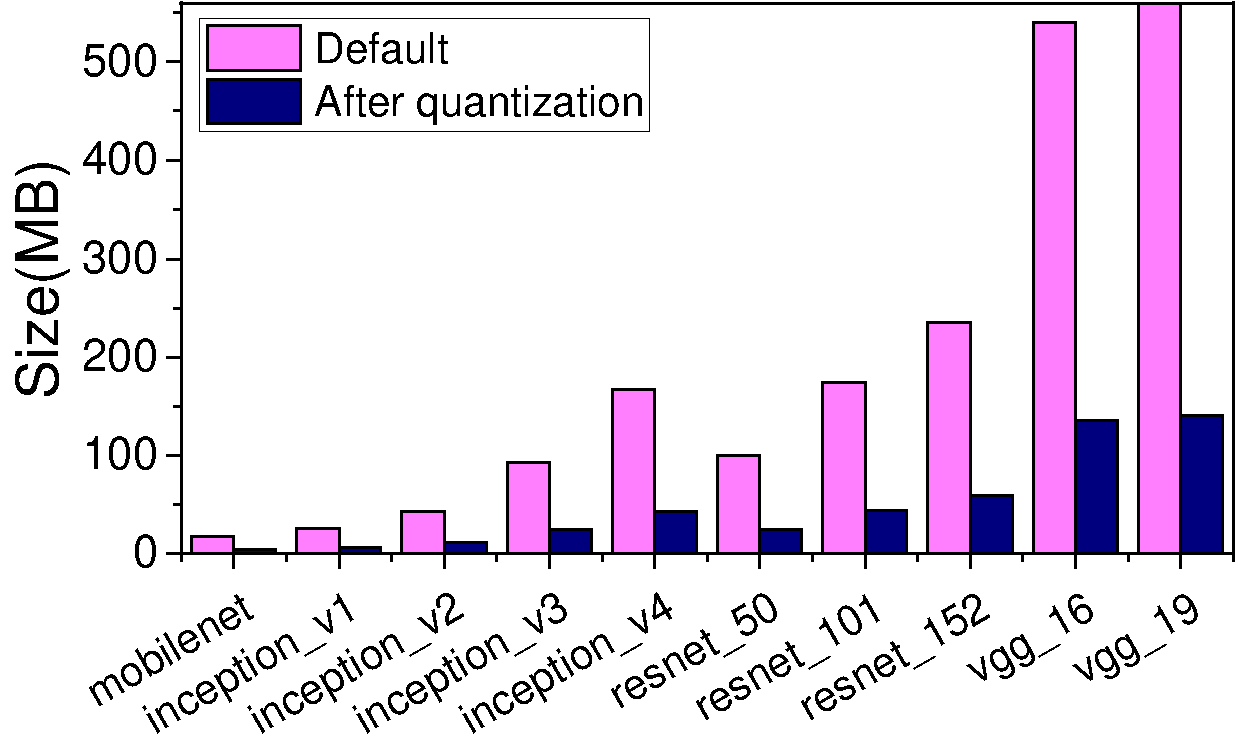
\includegraphics[width=0.33\textwidth]{figure/quan_size.pdf}}
\hfill
\subfloat[][Inference time]{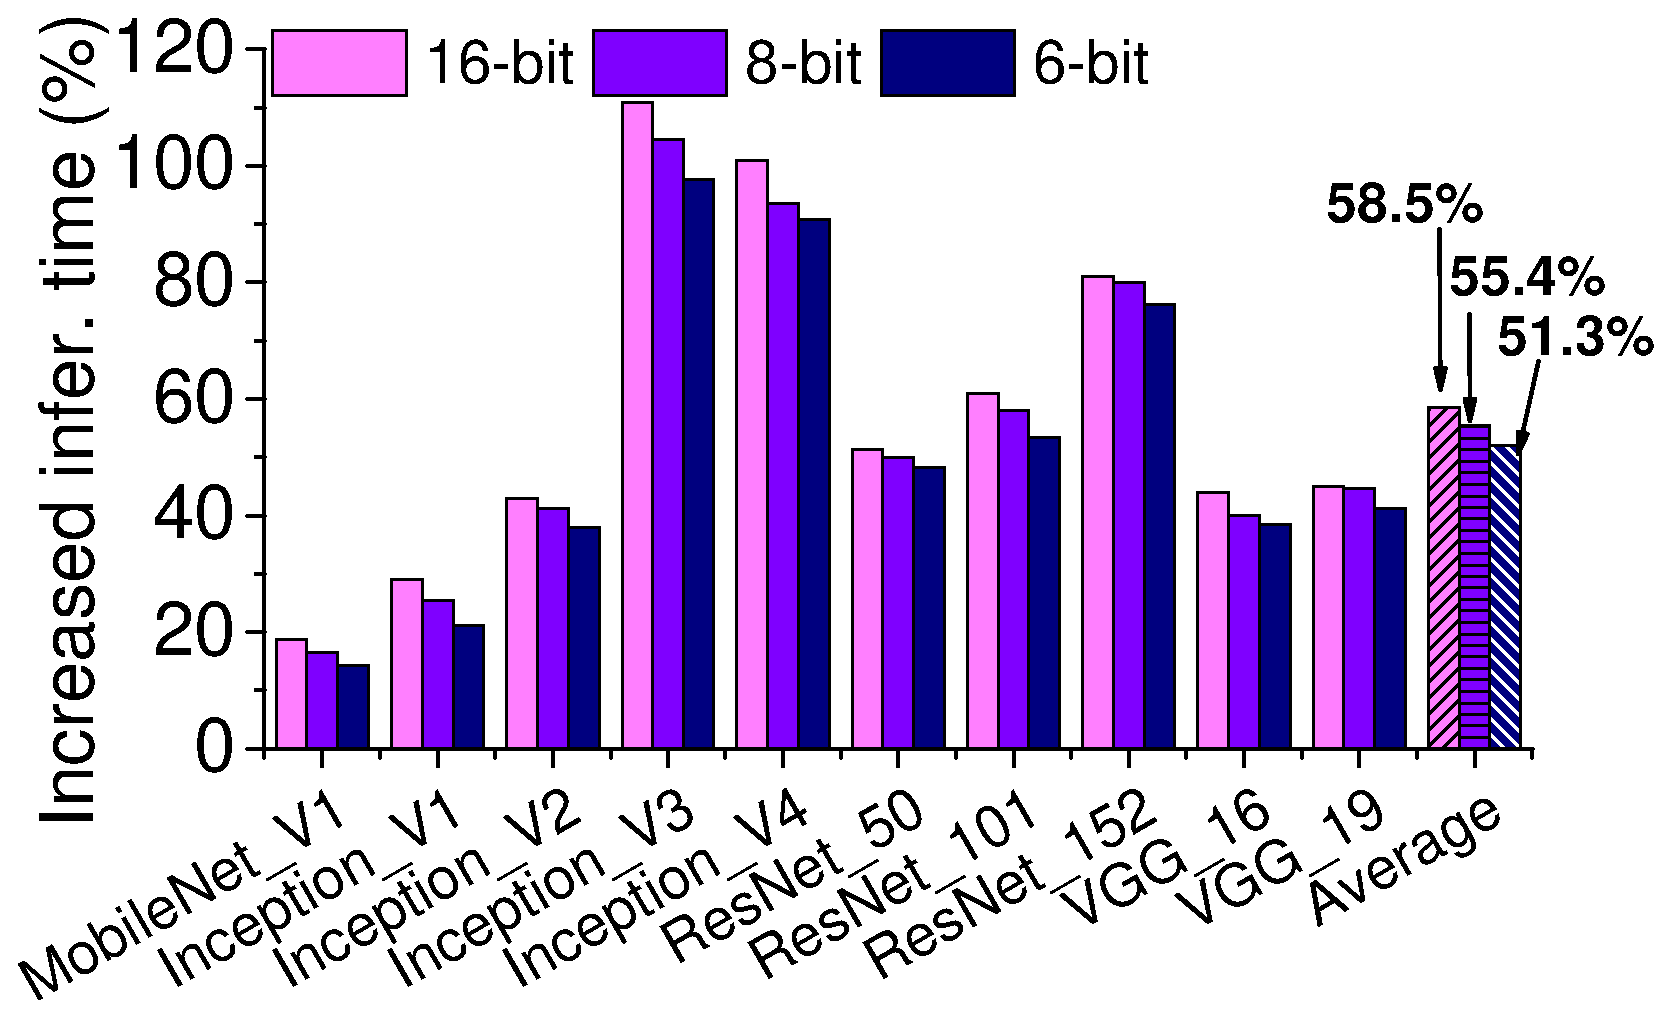
\includegraphics[width=0.34\textwidth]{figure/quan_time2.pdf}}
\hfill
\subfloat[][Accuracy]{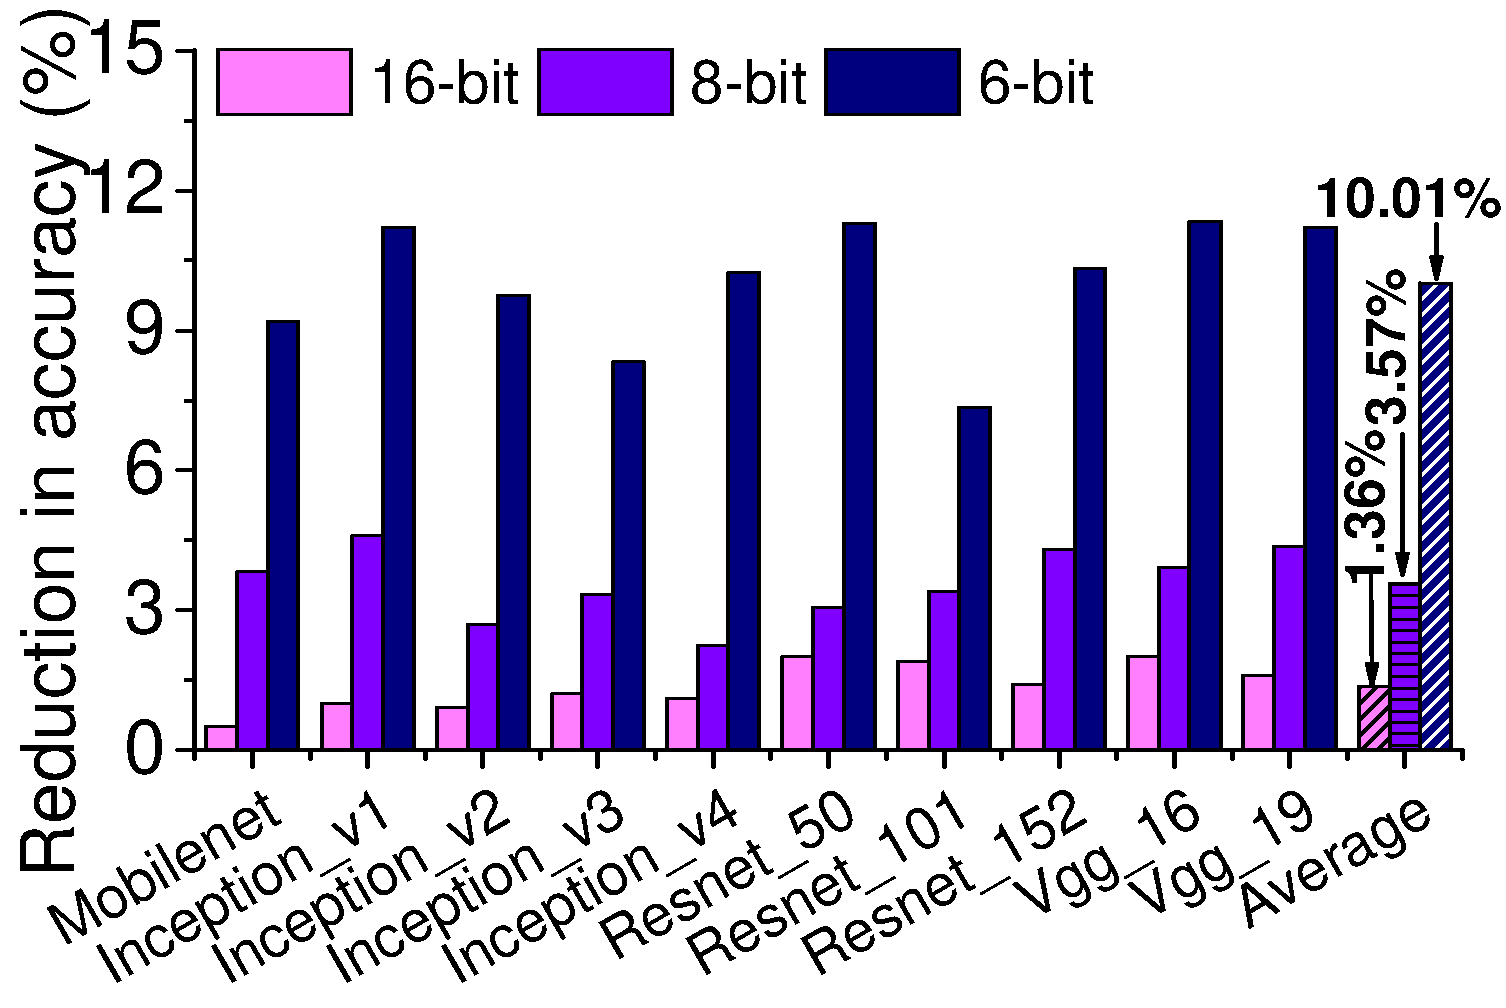
\includegraphics[width=0.32\textwidth]{figure/quan_acc3.pdf}}
\hfill
\subfloat[][Power consumption]{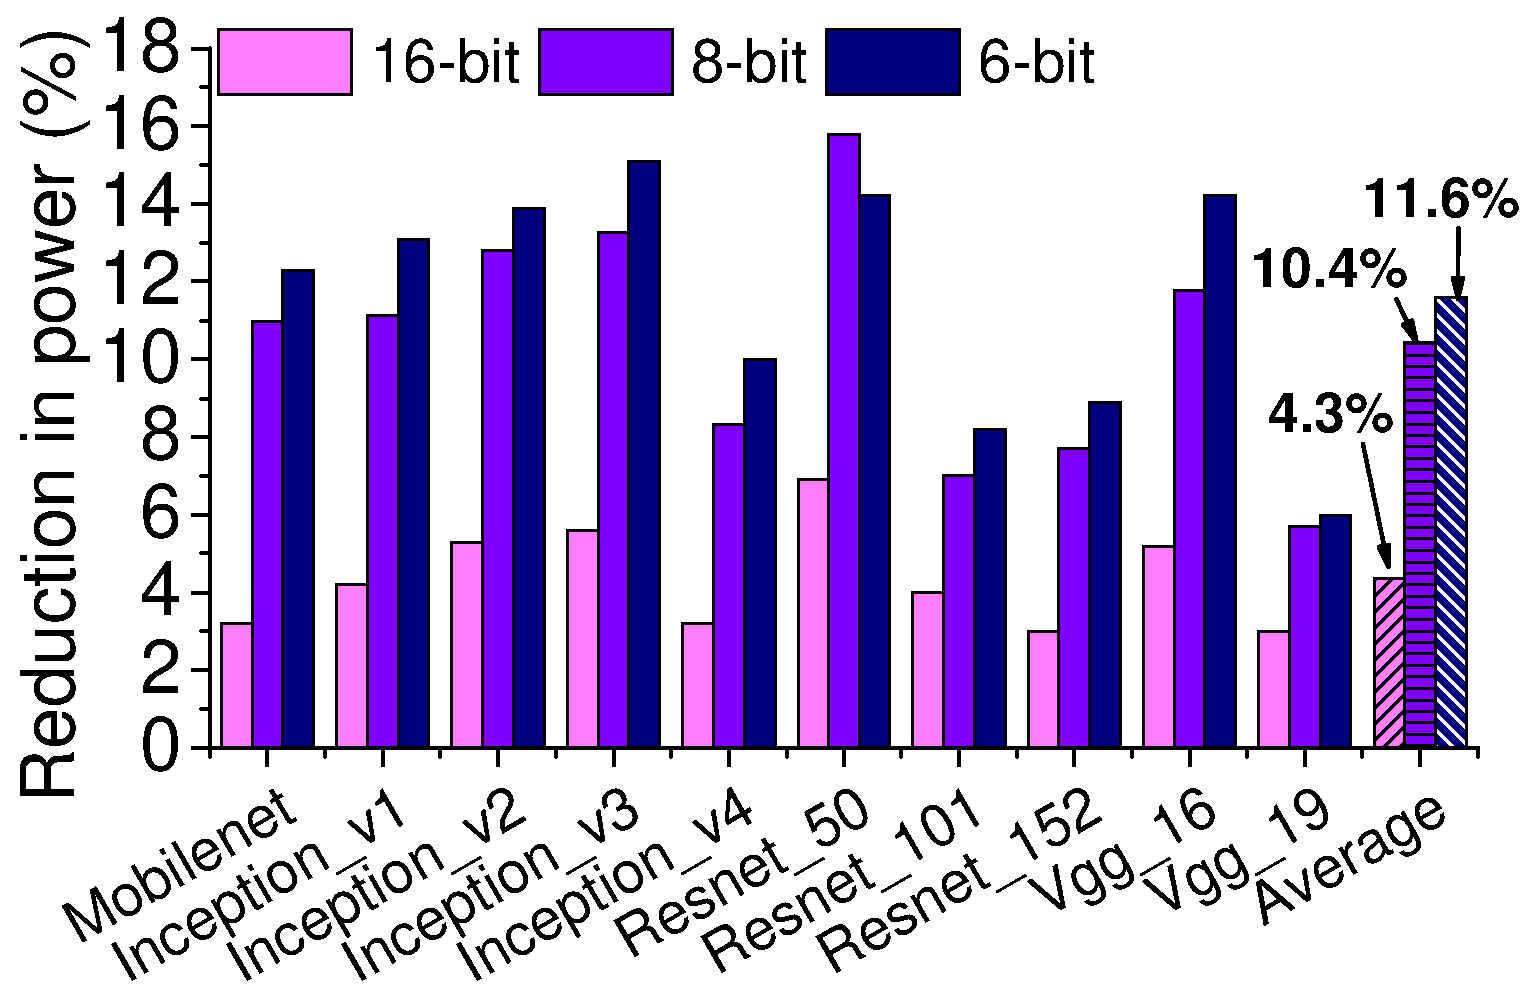
\includegraphics[width=0.33\textwidth]{figure/quan_power2.pdf}}
\hfill
\subfloat[][Energy consumption]{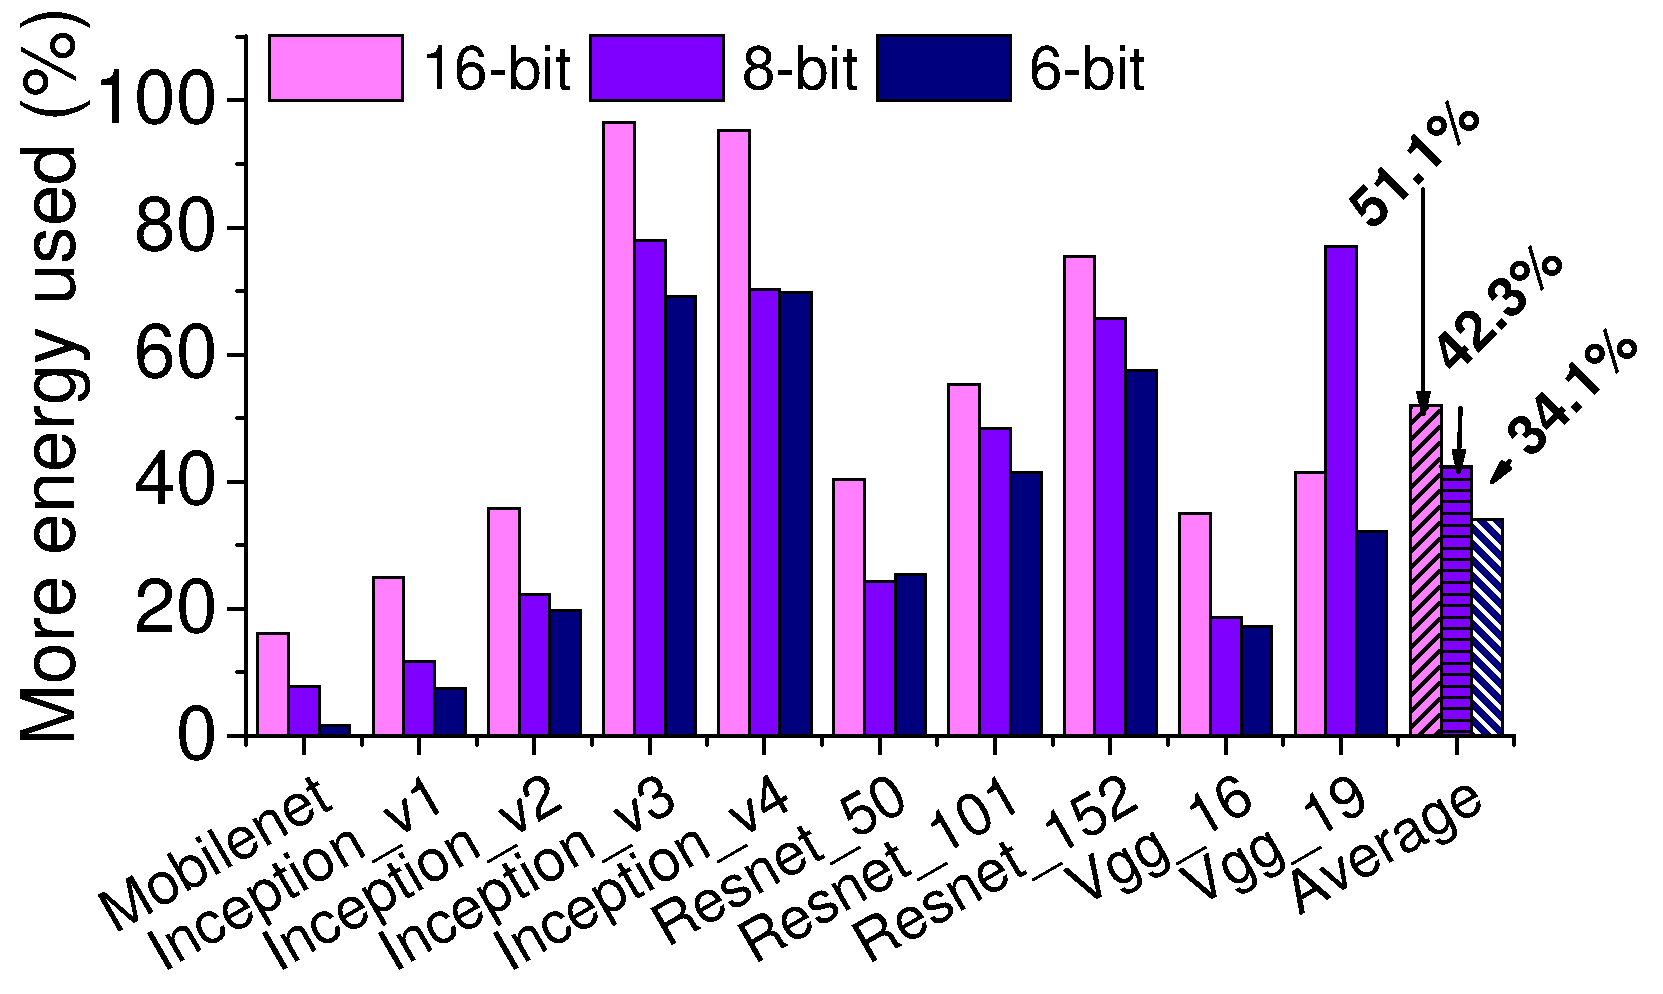
\includegraphics[width=0.34\textwidth]{figure/quan_energy2.pdf}}
\hfill
\subfloat[][precision, recall and F1 score]{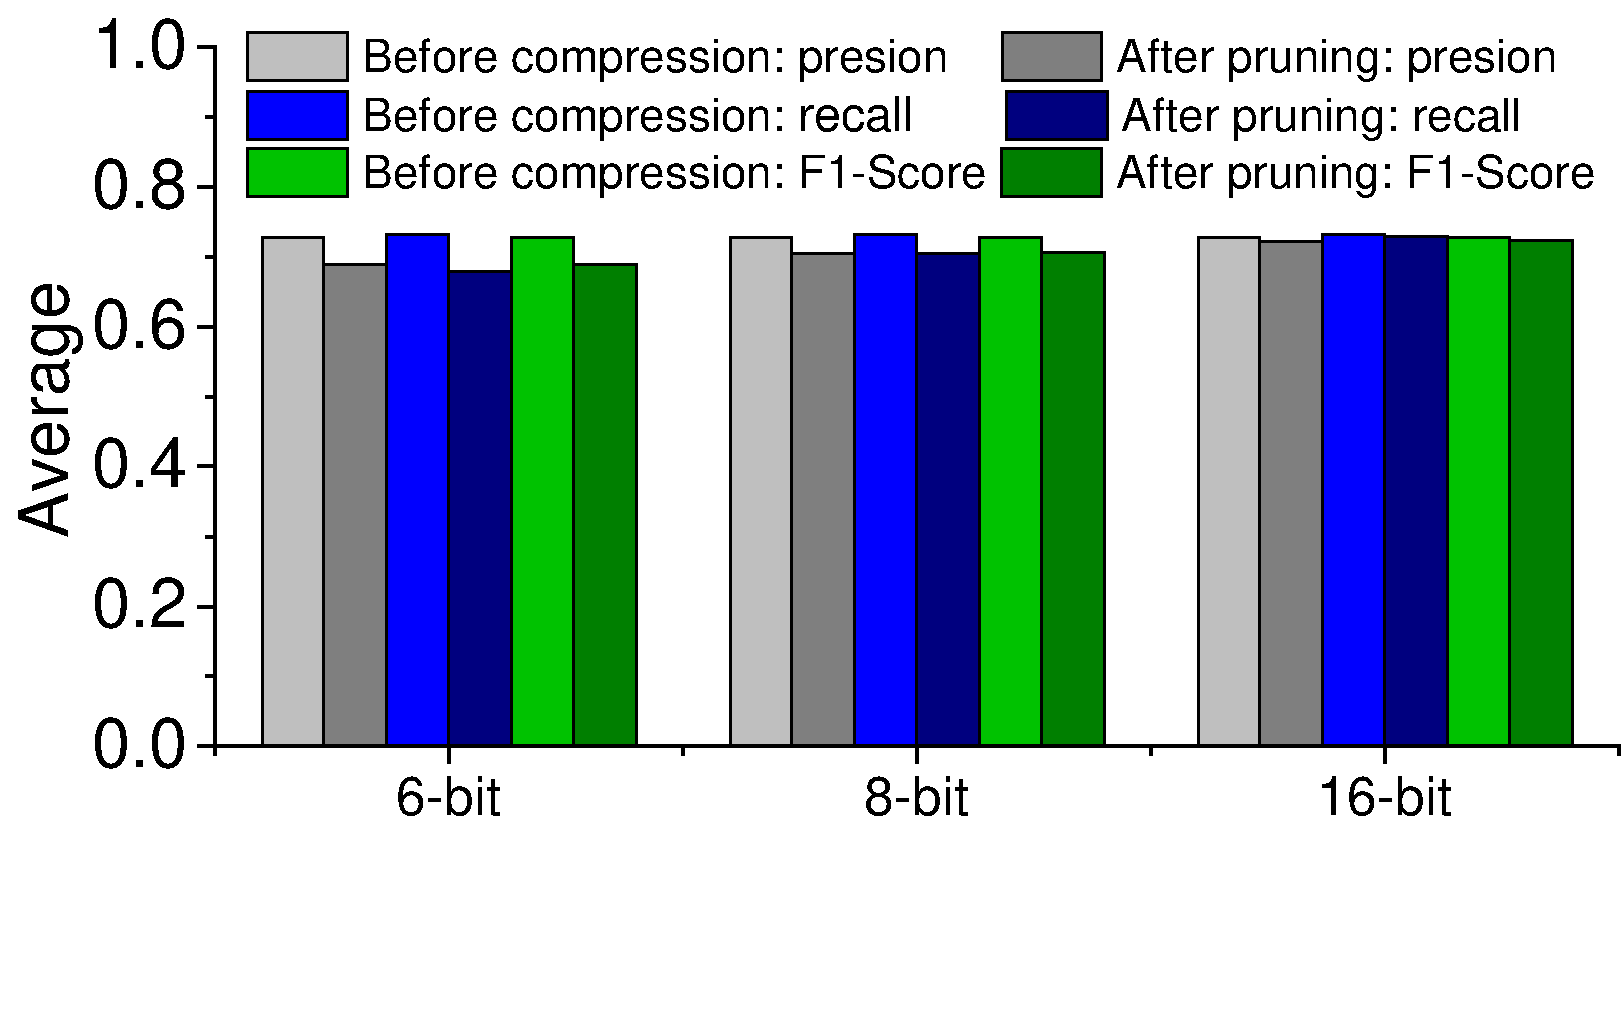
\includegraphics[width=0.33\textwidth]{figure/quan_prf2.pdf}}
\hfill

\caption{The achieved model size (a) inference time (b) accuracy (c) power consumption (d)
energy consumption (e) and precision, recall and F1 score (e) before and after the compression by \quantization.
The compression technique to use depends on the optimization target.}
\label{fig:analy_quan}
\end{figure*}


\begin{figure*}[!t]
\centering
\subfloat[][Model size]{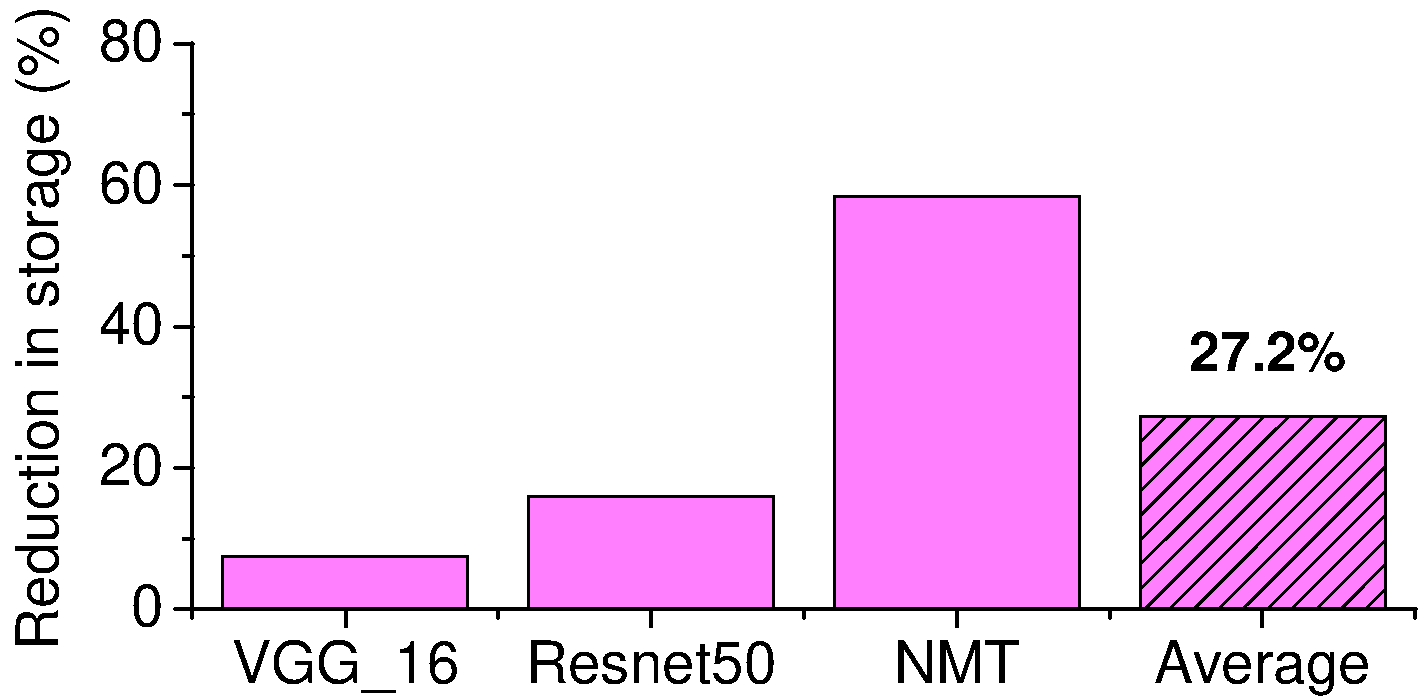
\includegraphics[width=0.33\textwidth]{figure/prun_size.pdf}}
\hfill
\subfloat[][Inference time]{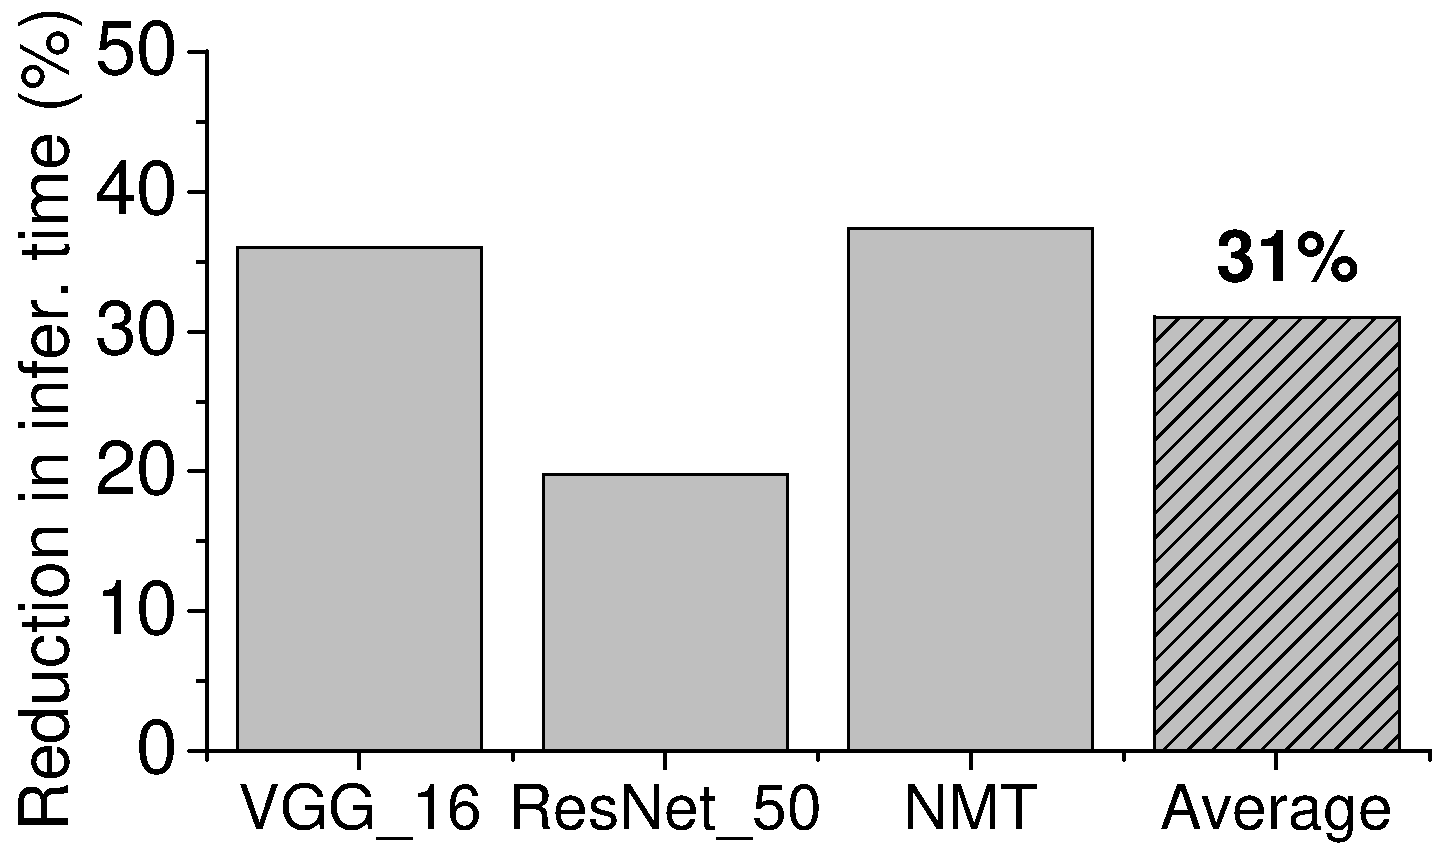
\includegraphics[width=0.3\textwidth]{figure/prun_time.pdf}}
\hfill
\subfloat[][Accuracy]{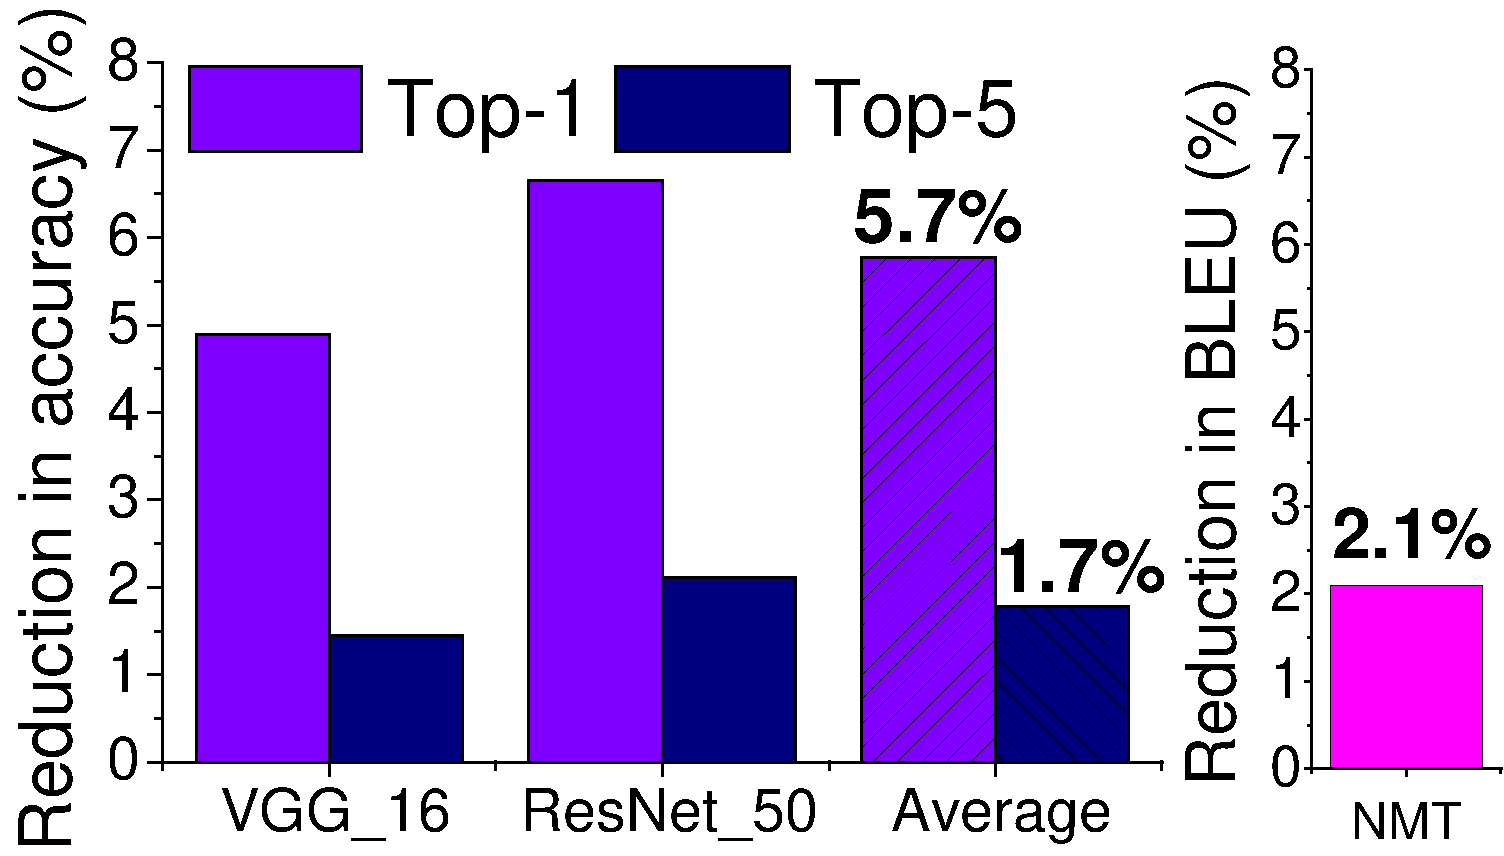
\includegraphics[width=0.3\textwidth]{figure/top1_5_prun.pdf}}
\hfill
\subfloat[][Power consumption]{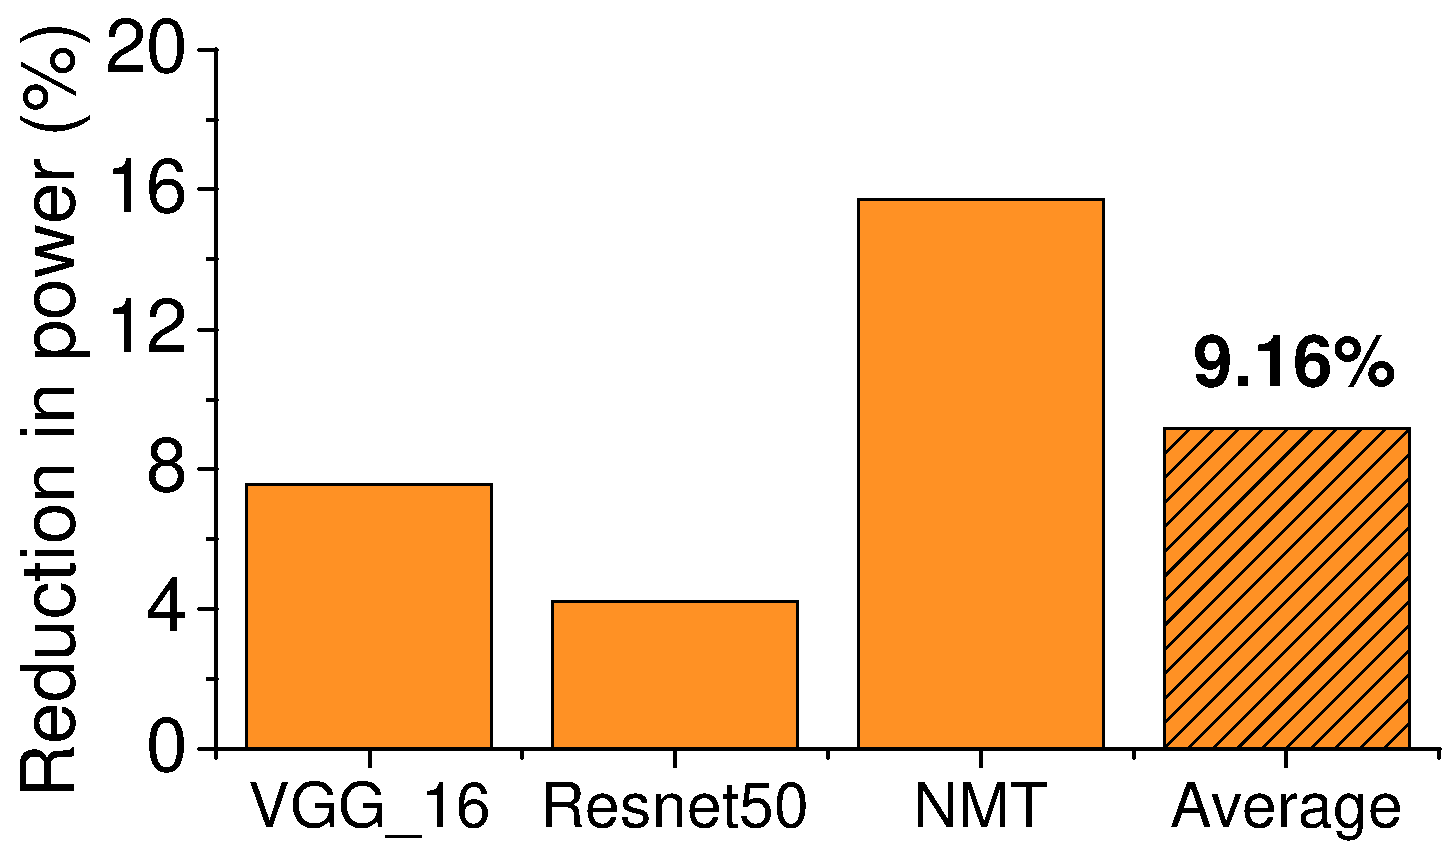
\includegraphics[width=0.3\textwidth]{figure/prun_power.pdf}}
\hfill
\subfloat[][Energy consumption]{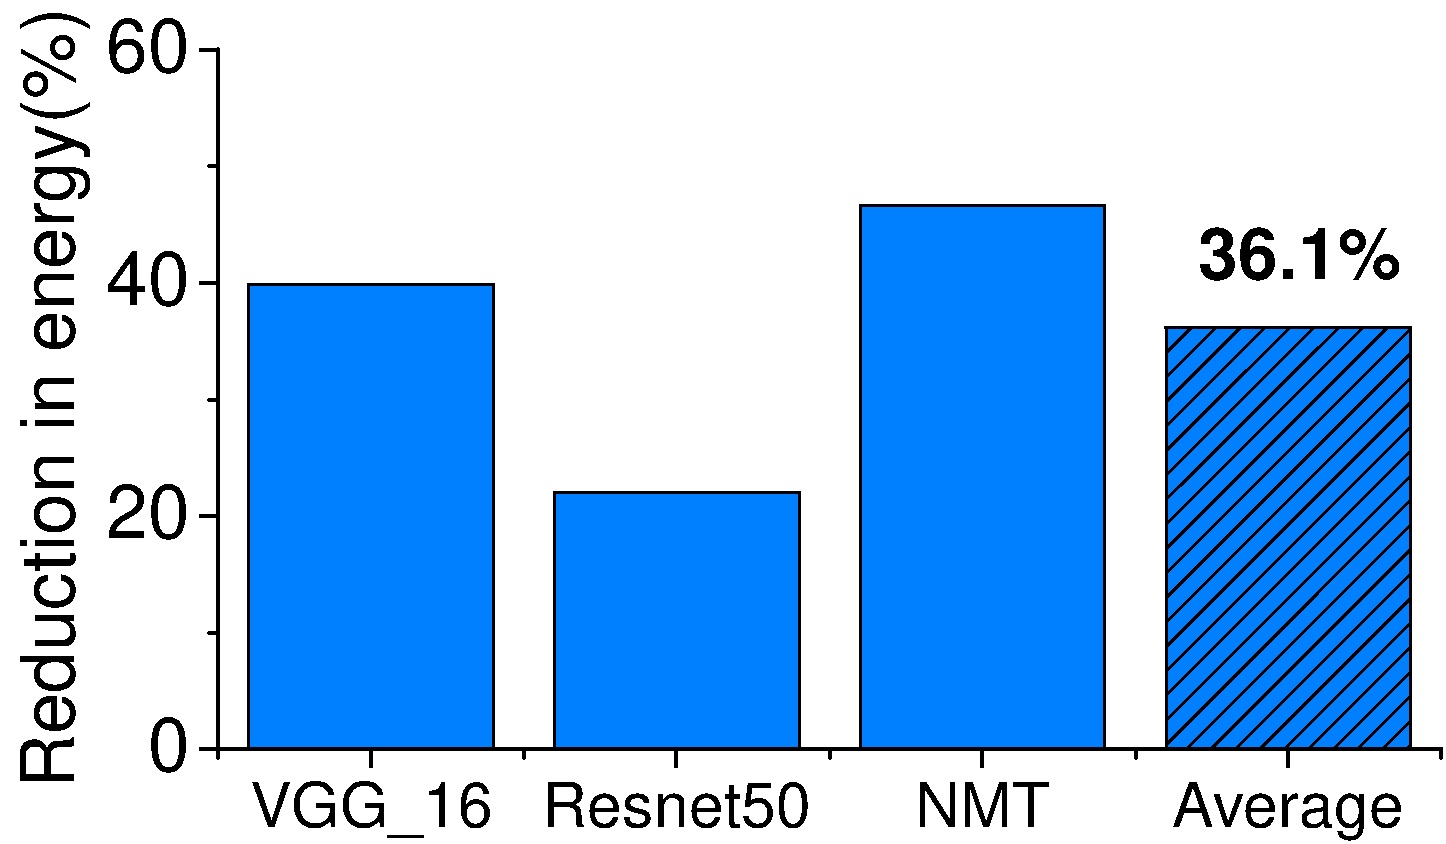
\includegraphics[width=0.3\textwidth]{figure/prun_energy.pdf}}
\hfill
\subfloat[][precision, recall and F1 score]{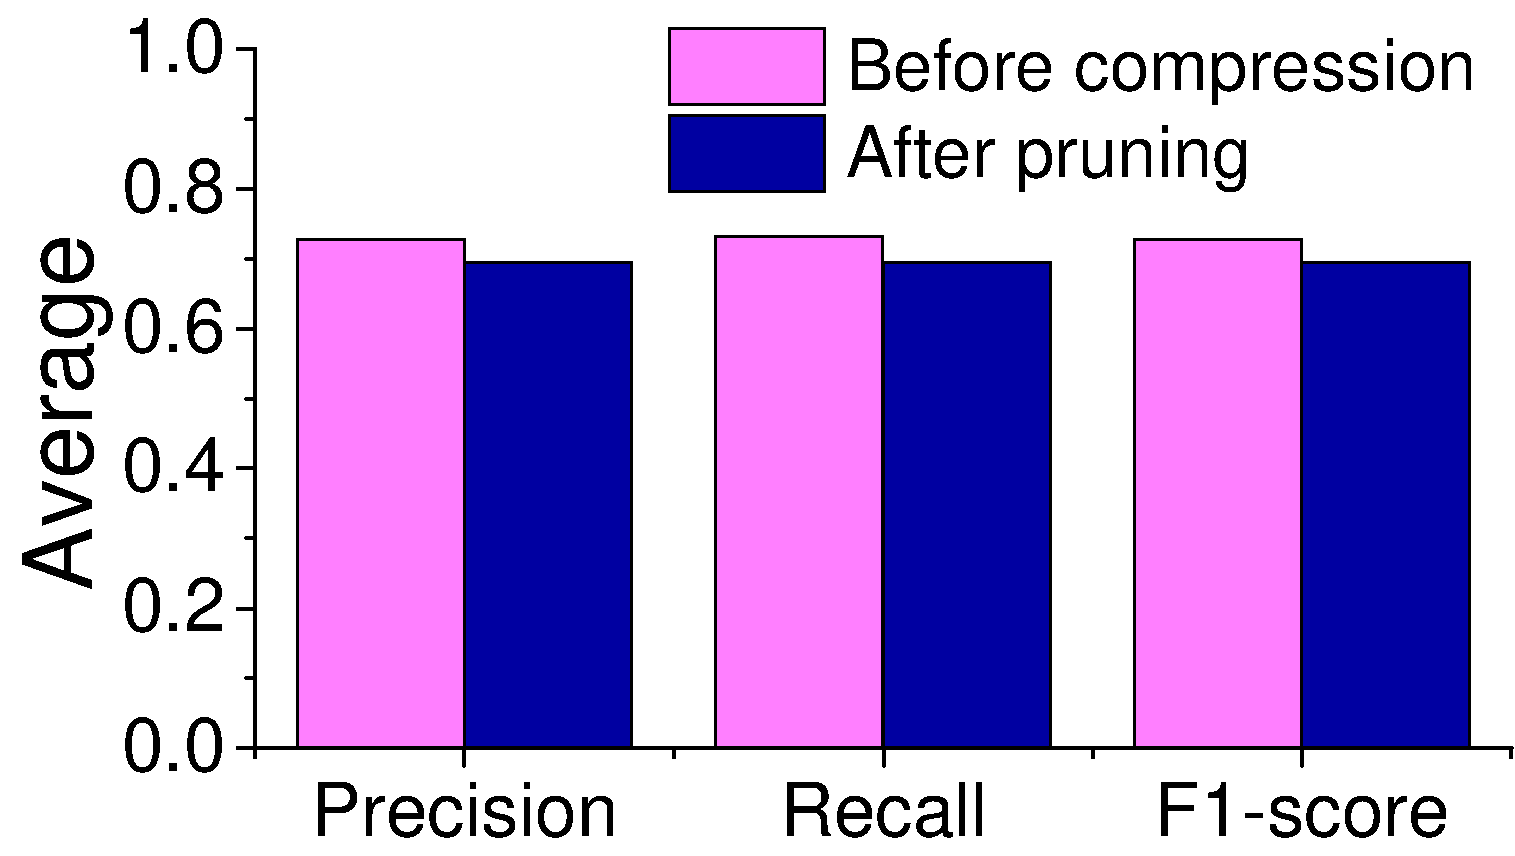
\includegraphics[width=0.3\textwidth]{figure/prun_prf.pdf}}
\hfill

\caption{The change of the model size (a), inference time (b), accuracy/BLEU (c), power (d), energy consumption (e), and accuracy (e)
before and after applying \pruning.} \label{fig:analy_prun}
\end{figure*}

\section{Experimental Results}


\subsection{Roadmap}
Our experiments try to answer the following questions:

\begin{itemize}
\item bla
\item bla2
\item bla3
\end{itemize}

\subsection{Impact on the Model Storage Size\label{sec:ms}}
Reducing the model storage size is crucial for embedded and IoT systems which often have a limited storage space. A smaller model size also
translates to smaller runtime memory footprint of less RAM space consumption. Figures~\ref{fig:analy_quan} and  \ref{fig:analy_prun}
illustrate how the different compression techniques and parameters affect the resulting model size.

As can be seen from Figure~\ref{fig:analy_quan}a, data quantization can significantly reduce the model storage size, leading to an average
reduction of 50.2\% when using a 16-bit representation and up to 80.7\% when using a 6-bit representation. The reduction in the storage
size is consistent across neural networks as the size of a network is dominated by its weights.

From Figure~\ref{fig:analy_prun}a, we see that by removing some of the pathways of the neural network, \pruning can also reduce the model
size, although the gain is smaller than \quantization. On average, \pruning reduces the model size by 27.2\% (49.26 MB). An interesting
observation is that, \pruning is particularly effective for obtaining a compact model for NMT, an \RNN, with a reduction of 60\% on the
model size. This is because there are typically many repetitive pathways in an \RNN due to the natural of the network architecture. As we
will discuss later, \pruning only leads to a minor degradation in the prediction accuracy for NMT. This suggests that \pruning can be an
effective model compression technique for \RNNs.



\subsection{Impact on Inference Time}
 Figure~\ref{fig:analy_quan}b compares the inference time when using different bit
widths to represent a 32-bit floating number for neural network weights. Intuitively, a smaller model should run faster. However, data
quantization does not reduce the inference time but instead it prolongs it. Data quantization can speedup the computation (i.e., matrix
multiplications) performed on the input data by avoiding expensive floating point arithmetics and enabling SIMD vectorization by using a
compact data representation. However, we found that the overhead of the quantization process during inference can outweigh its benefit.
Except the genernal inference operation, a data quantization and de-quantization function has to be added into the compressed model. The quantization function converts the 32-bit to quantized weights, after inference operation which
accounts for 50.9\%, the de-quantization quantized
weights back to a 32-bit representation on the output layer to recover the loss in precision. As can be seen from Figure~\ref{fig:breakdown}, this process could be expensive, contributing to 30\% to 50\% of the end to end inference time.
%this process could be expensive, contributing to 30\% to 50\% of the end to end inference time.
%After data quantization, a de-quantization function has to be added into the compressed model. This  function converts %the quantized
%weights back to a 32-bit representation on the output layer to recover the loss in precision. As can be seen from %Figure~\ref{fig:breakdown},
%this process could be expensive, contributing to 30\% to 50\% of the end to end inference time.

\begin{figure}
\begin{center}
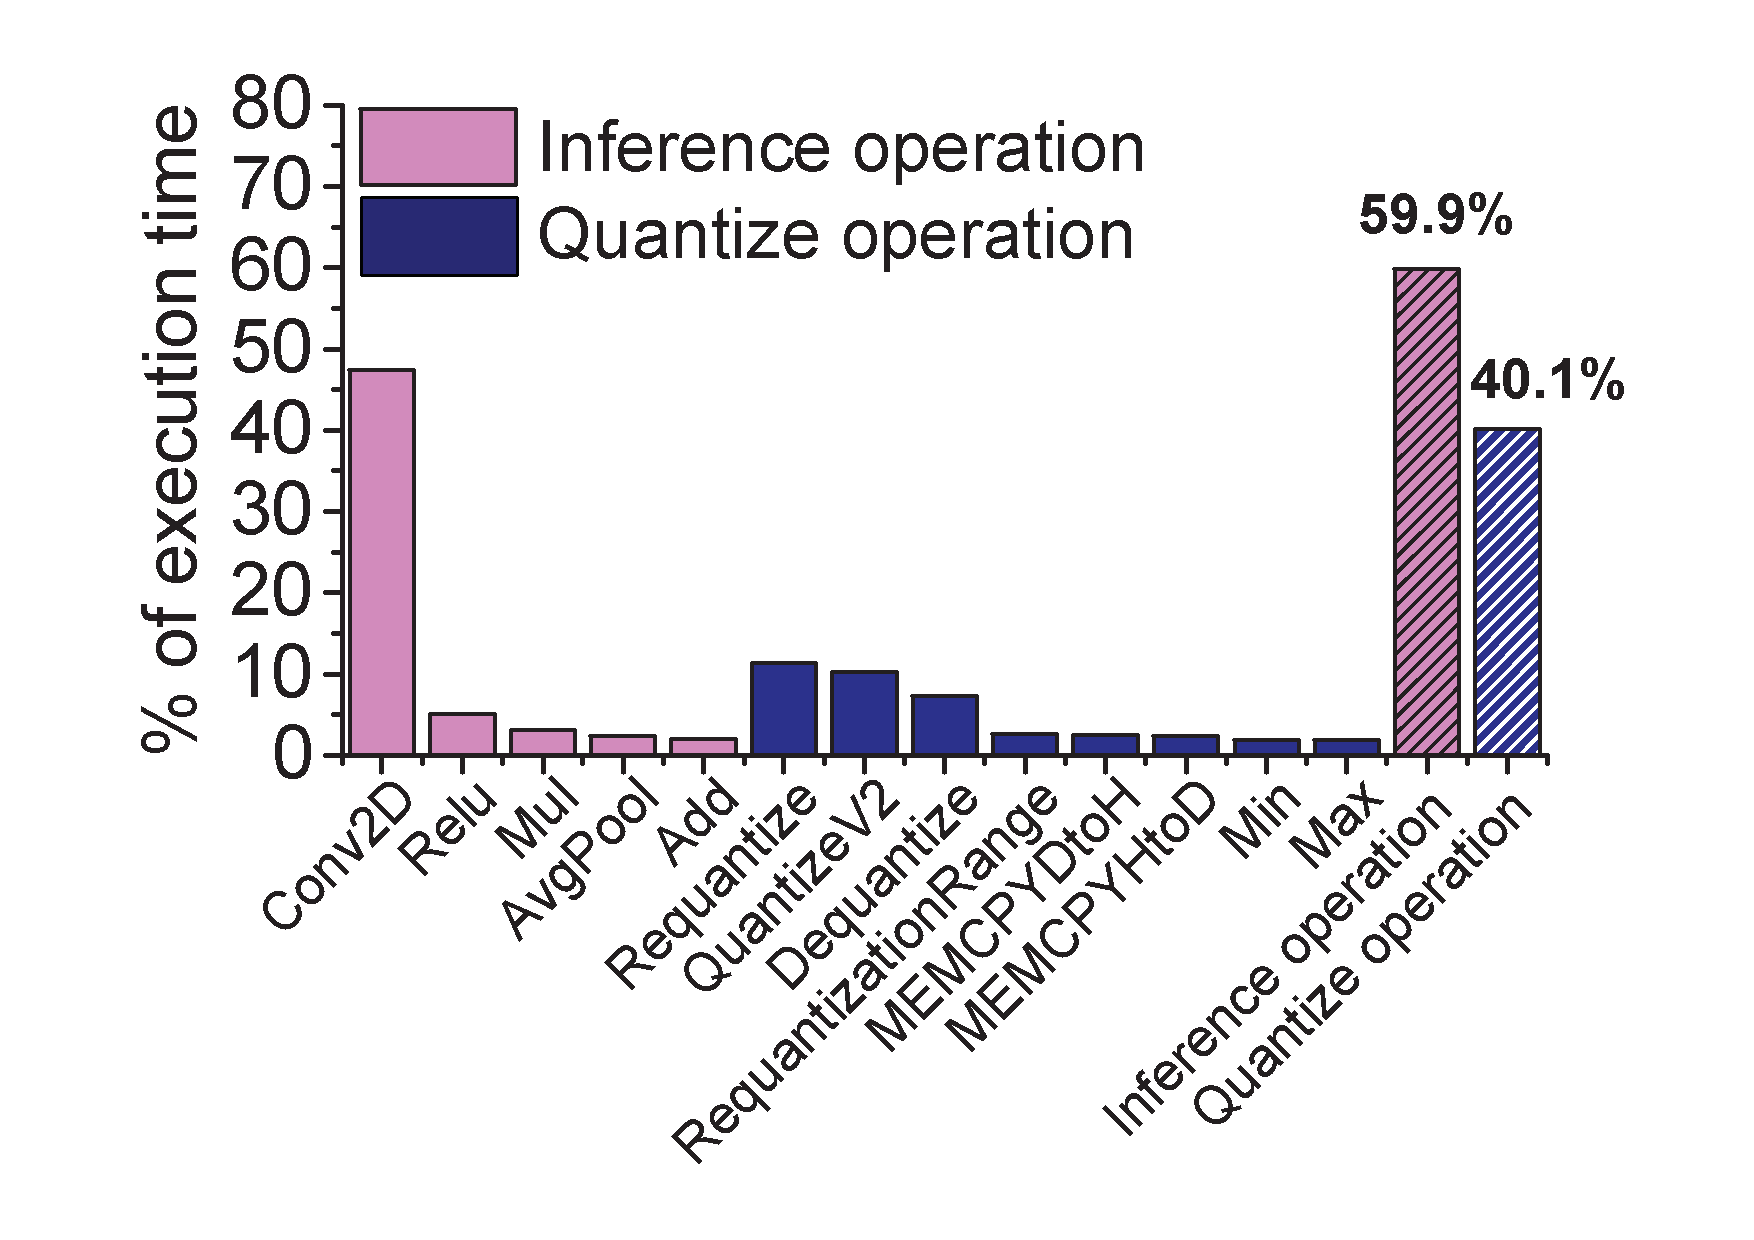
\includegraphics[width=0.48\textwidth]{figure/breakdown2.pdf}
\end{center}
\caption{Breakdown of average execution time by operation type for ten models.}
\vspace{-2mm}
\label{fig:breakdown}
\end{figure}


Using fewer bits for representation can reduce the overhead of de-quantization. For example, using a 6-bit representation is 1.05x and
1.03x faster than using a 16-bit and a 8-bit representations, respectively. However, as we will demonstrate later when discussing
Figure~\ref{fig:analy_quan}c, using fewer bits has the drawback of causing larger degradation in the prediction accuracy. Hence, one must
carefully find a balance between the storage size, inference time, and prediction accuracy when applying data quantification.

We also find that the percentage of increased inference time depends on the neural network structure. Applying data quantization to
\texttt{Inception}, the most complex network in our \CNN tested set, will double the inference time. By contrast, data quantization only
leads to a 20\% increase in inference time for \texttt{Mobilenet}, a compact model. This observation suggests that data quantization may be
beneficial for simple neural networks on resource-constrained devices.


In contrast to \quantization, Figure~\ref{fig:analy_prun}b shows that \pruning leads to faster inference time across evaluated networks. We
can see that the inference time of \texttt{Vgg\_16} and \texttt{NMT} can benefit from this technique, with an reduction of 38\%.  Overall,
the average inference time is reduced by 31\%. This suggests that while \pruning is less effective in reducing the model size (see
Section~\ref{sec:ms}), it can be useful in achieving a faster inference time.


\subsection{Impact on Accuracy Metrics}
In addition to the storage size and inference time, accuracy is crucially important for a predictive model. A small and faster model is not
very useful if it gives wrong predictions all the time.


Results in Figure~\ref{fig:analy_quan}c compare how the prediction accuracy is affected by model compression. We see that the sweat spot of
\quantization depends on the neural network structure. An 16-bit representation keeps the most information of the original model and thus
leads to little reduction in the prediction accuracy, on average  1.36\%.  Using an 8-bit representation would lead on average 3.57\%
decrease in the accuracy, while using a 6-bit representation will lead to a significantly larger reduction of 10\% in  accuracy. We also
observe that some networks are more robust to \quantization. For example, while a 6-bit representation leads to less than 10\% decrease in
accuracy for \texttt{Resnet\_101}, it cause a 12\% drops in accuracy for \texttt{Resnet\_50}. This is because a more complex network (i.e.,
\texttt{Resnet\_101} in this case) is more resilient to the weight errors compared to network (i.e., \texttt{Resnet\_50} in this case) with
a smaller number of layers and neurons. Our findings suggest the need for having an adaptive scheme to choose the optimal \dquantization
parameter for given constraints.


For \pruning, the Figure~\ref{fig:analy_prun}c compares the reduction in the top-1 and the top-5 accuracies for \texttt{Vgg\_16} and
\texttt{Resnet\_50}. We also show the BLEU value for \texttt{NMT}. \pruning reduces the accuracy of the two \CNN models with by 5.7\% and
1.7\% respectively for the top-1 and top-5 scores. We observe that the \pruning has little negative impact on \texttt{NMT} where we only
observe an averaged loss of 0.8\% for BLEU. When taking into consideration that \pruning can significantly reduce the model size for
\texttt{NMT} (Section~\ref{sec:ms}), our results suggest that \pruning is particularly effective for \RNNs.


%Although an 8-bit representation leads to a minor
%decrease in the prediction accuracy, a further reduction of a 6-bit representation is only profitable for xx networks.



\subsection{Impact on the Power and Energy Consumption}
Power and energy consumption are two limiting factors on battery-powered mobile and IoT devices. As we can see from
Figure~\ref{fig:analy_prun}d, \quantization decreases the peak power for inferencing with an average of 4.3\%, 10.4\% and 11.6\%,
respectively when using a 6-bit, an 8-bit and a 16-bit representations. While \quantization reduces the peak power used, the increase
inference time leads to more energy consumption by at least 34.1\% and up to 51.1\% (see Figure~\ref{fig:analy_prun}e). This means that
although \quantization allows one to reduces voltage supply to the computing devices, it can lead to a short battery life.

Figure~\ref{fig:analy_prun}e shows the reduced energy consumption by applying \pruning. Note that it saves over 40\%, 15\% and 50\% energy
consumption for \texttt{Vgg\_16}, \texttt{Resne\_50} and \texttt{NMT} respectively. Despite that the peak power is reduced by only 9.16\%,
a smaller decrease compared to \quantization, the resulted faster inference time allows \pruning to significantly reduce the power
consumption. The results suggest \pruning is useful for reducing the overall energy consumption of the system, but \quantization can be
employed to support a low power system.



\subsection{Precision, Recall and F1-Score}

Finally, Figure~\ref{fig:analy_quan}f and 
Figure~\ref{fig:analy_prun}f show other three evaluation metrics of these models 
after \quantization and \pruning. We can see that, the compressed models only violate
less than 3\% for precision, recall and F1-Score. 
For \quantization, the 16-bit representation outperforms the other two bits width respresentations.
Specifically, 16-bit gives the
highest overall precision, which in turns leads to the best F1
score. High precision can reduce false positive, which is
important for certain domains like video surveillance
because it can reduce the human involvement for inspecting
false positive predictions.




\subsection{Memory footprint}

\begin{figure}[!t]
\centering
\subfloat[][\quantization]{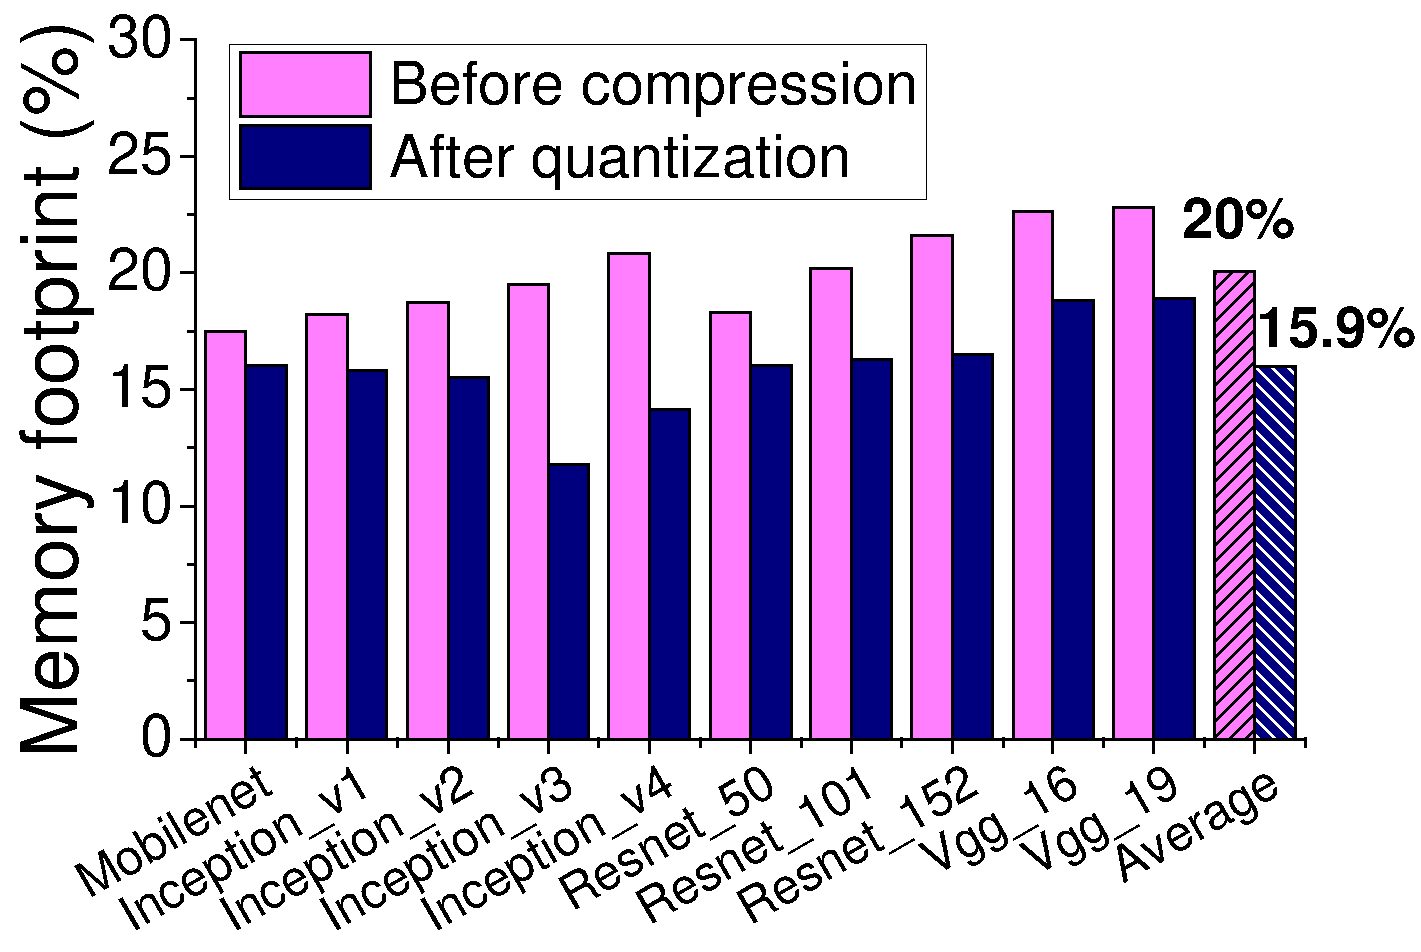
\includegraphics[width=0.4\textwidth]{figure/quan_mem.pdf}}
\hfill
\subfloat[][\pruning]{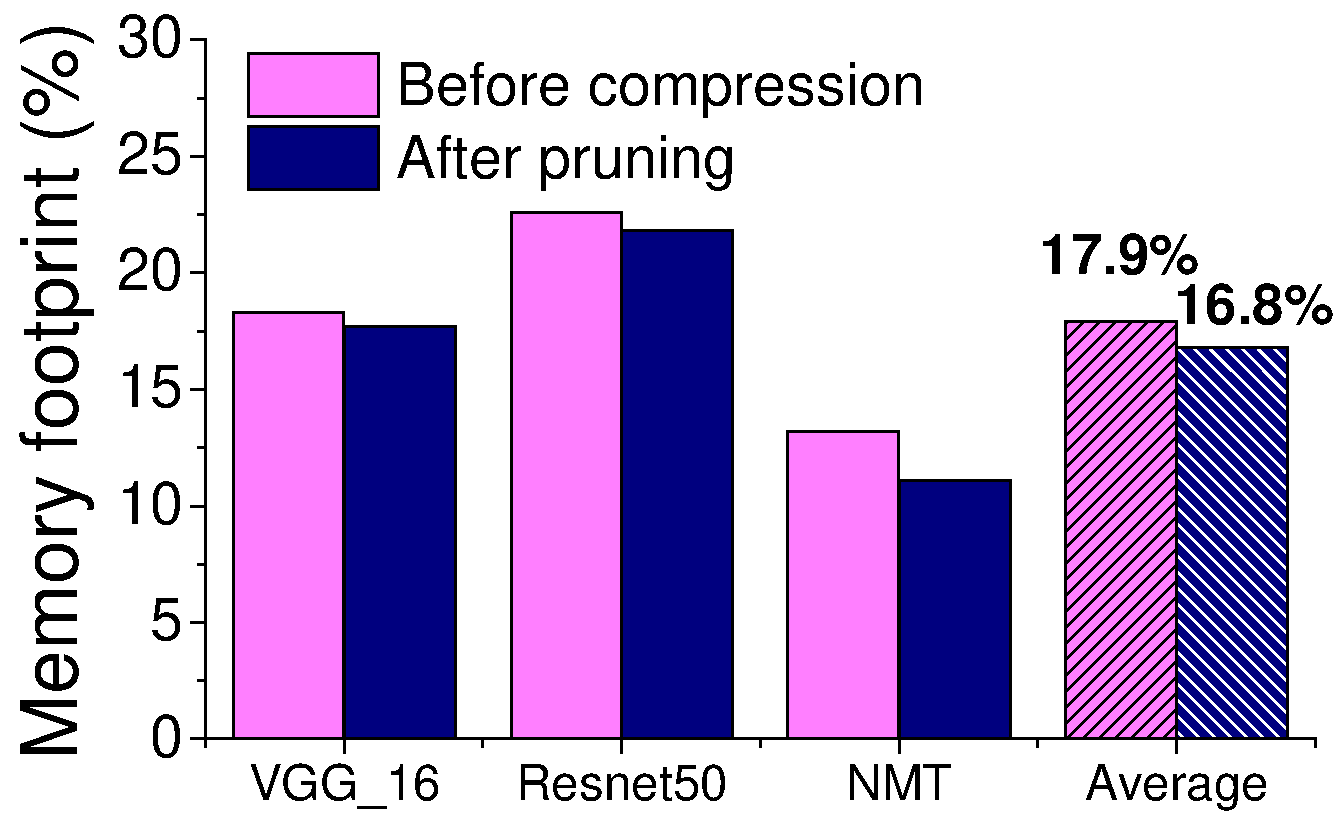
\includegraphics[width=0.4\textwidth]{figure/prun_mem.pdf}}
\hfill

\caption{Memory footprint before and after the compression by \quantization(a) and \pruning (b).}
\label{fig:footprint}
\end{figure}

Figure~\ref{fig:footprint} compares the resulting memory footprint by applying \quantization and \pruning. Quantization reduces the runtime
memory footprint with an averaged reduction of 17.2\% by generating a more compact model. For example, an 8-bit representation reduces the
memory footprint from 20.02\% to 15.97\% across networks, with an averaged reduction of 20.63\% (up to 40\%). In general, the smaller the
model storage size is, the less memory footprint the compressed model will be. As an example, a 6-bit representation uses \FIXME{xx, and
xx} less memory compared to a 8-bit and a 16-bit representations, respectively.

In contrast to \dquantization, Figure~\ref{fig:footprint} shows that  \pruning offers little help in reducing the model memory footprint.
On average, it leads to a 6.4\% reduction of memory footprint. This is because that the network weights still domain the memory resource
consumption, and \pruning is less effective compared to \dquantization for reducing the overhead of network weights.


\subsection{Compare to Oracle.} 

\begin{figure}[!t]
\centering

\subfloat[][\quantization]{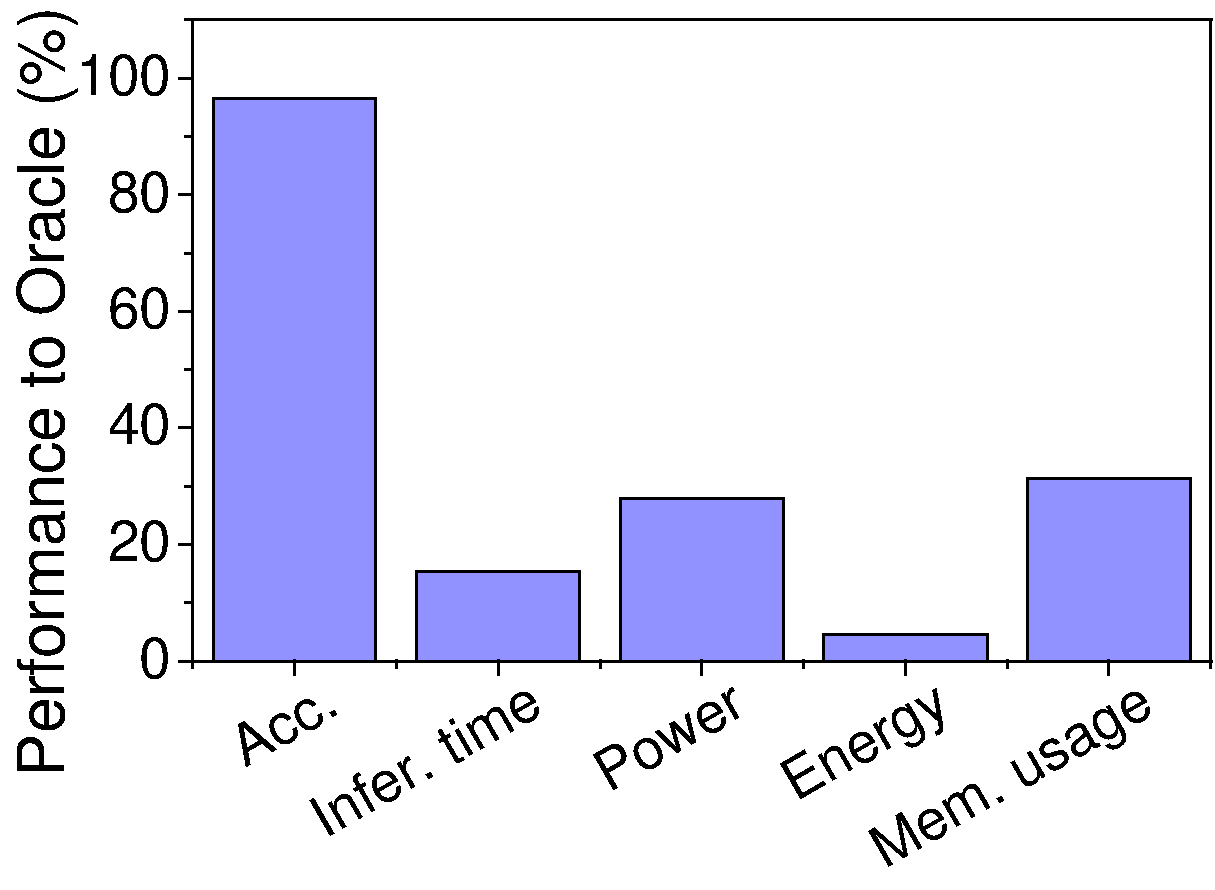
\includegraphics[width=0.35\textwidth]{figure/quan_oracle.pdf}}
\hfill
\subfloat[][\pruning]{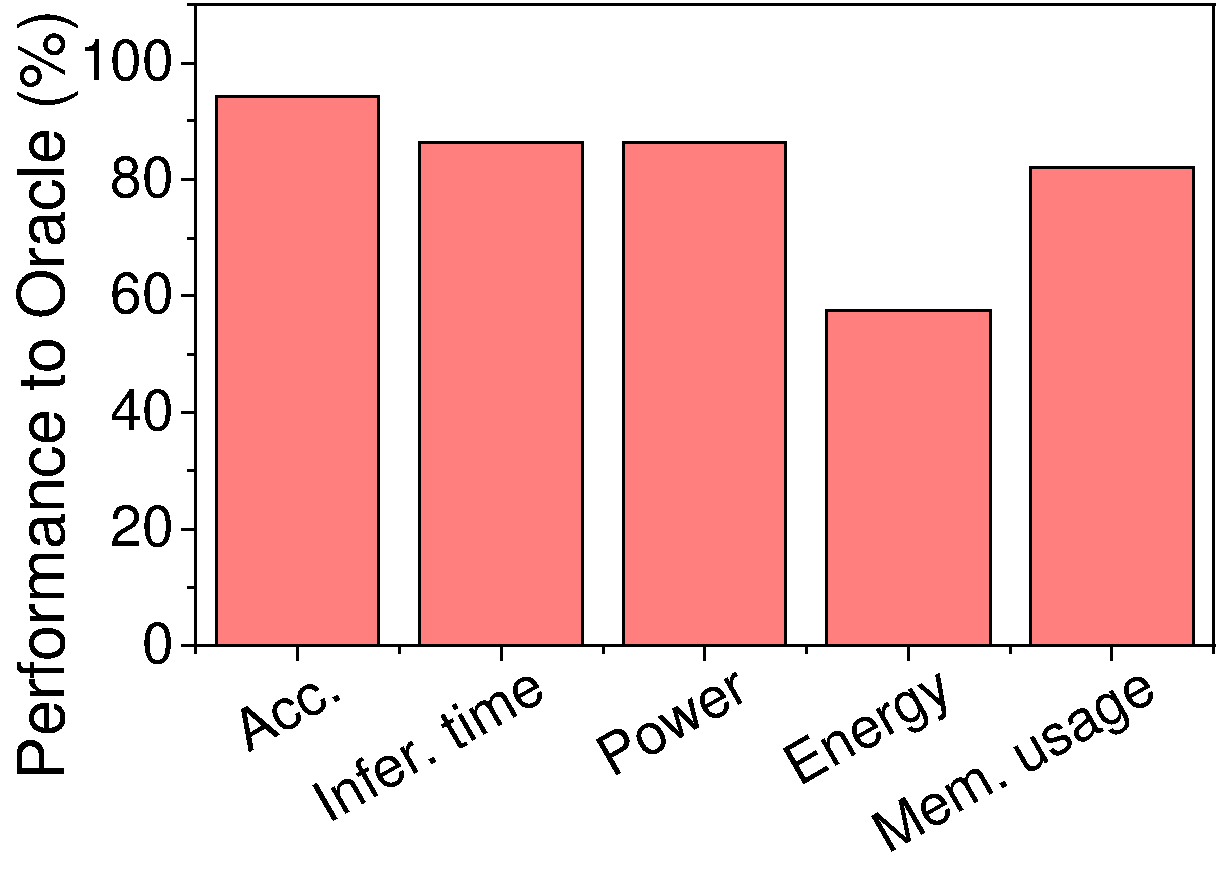
\includegraphics[width=0.35\textwidth]{figure/prun_oracle.pdf}}
\hfill

\caption{Our compressed models' performance w.r.t. performance of an oracle performance for \quantization (a) and \pruning (b).}
\label{fig:oracle}
\end{figure}

In Figure~\ref{fig:oracle}, we compare our compressed models to ideal compressed models. 
We set the 8-bit data quantization as the ideal quantized weight, as it offers an affordable 
accuracy after quantization. Note that, the accuarcy almost achieves the ideal value, on the contary,
the inference time and enery consumption perform worst, only account less than 10\%. Bot of 
the inference time and memory usage occupy more than 20\%.
Figure~\ref{fig:oracle} b presents the how close our pruned models to the theoretically 
perfect models. As we can see from this figure, most of evaluation metrics above 80\%,
and the energy consunsumption also achieves 58\%.





\section{Related Work}
\DNNs have shown astounding successes in various tasks that previously seemed difficult~\cite{}. Despite the fact that many embedded
devices require precise sensing capabilities, adoption of \DNN models on such systems has notably slow progress. This mainly due to
\DNN-based inference being typically a computation intensive task, which inherently runs slowly on embedded devices due to limited
resources.

\FIXME{Talk about different compression techniques.}

There is an extensive body of work on how to accelerate \DNN training using xx, xx, and xx. Our work aims to understand how to accelerate
deep learning inference by choosing the right model compression technique.


As an alternative to on-device inferencing, off-loading computation to the cloud can accelerate \DNN model inference
\cite{teerapittayanon2017distributed}. Neurosurgeon \cite{Kang2017neurosurgeon} identifies when it is beneficial (\eg in terms of energy
consumption and end-to-end latency) to offload a \DNN layer to be computed on the cloud. The Pervasive \CNN~\cite{7920809} generates
multiple computation kernels for each layer of a \CNN, which are then dynamically selected according to the inputs and user constraints. A
similar approach presented in \cite{RodriguezWZMH17} trains a model twice, once on shared data and again on personal data, in an attempt to
prevent personal data being sent outside the personal domain. Computation off-loading is not always applicable due to privacy, latency or
connectivity issues. The work presented by Ossia \etal partially addresses the issue of privacy-preserving when offloading \DNN inference
to the cloud ~\cite{ossia2017hybrid}. Our work is complementary to prior work on computation off-loading by offering insights to choose the
optimal compression technique to best optimize local inference.

\section{Conclusions}
This paper has presented an automatic approach to optimize the mobile web



\bibliographystyle{IEEEtran}
\bibliography{IEEEabrv,refs}


% that's all folks
\end{document}


